\documentclass{cta-author}
\newtheorem{theorem}{Theorem}{}
\newtheorem{corollary}{Corollary}{}
\newtheorem{remark}{Remark}{}


% correct bad hyphenation here
\hyphenation{op-tical net-works semi-conduc-tor}
\usepackage[utf8]{inputenc}
\usepackage{graphicx}
\graphicspath{ {images/} }
%\usepackage{cite}
\usepackage{longtable}
\usepackage{amsmath}
\usepackage{multirow}
\usepackage{wrapfig}
%\usepackage{float}
%\usepackage[section]{placeins}
\usepackage{subcaption}
\usepackage{array}
\usepackage[export]{adjustbox}
%\usepackage{natbib}
\usepackage{tabu}
\usepackage{booktabs}
\usepackage[colorlinks=black,bookmarks=black,pdfborder={0 0 0},% this for auto cross reference
    linkcolor=black,urlcolor=black,citecolor=black,
    breaklinks=true,bookmarksnumbered=true]{hyperref}


\begin{document}

\title{Controller Hardware-In-the-Loop (CHIL) Testing of Fuzzy Logic Based Energy Storage Management System for Electric Ship}
\begin{abstract}
In this paper, a controller hardware-in-the-loop (CHIL) testing of a fuzzy logic (FL) based energy storage management (ESM) system of medium voltage DC (MVDC) power system of an all electric ship (AES) is presented. The incorporation of the pulsed load to the electric ship creates challenges for energy management on the shipboard power system. In order to facilitate the generators in meeting transient and steady power demand of the shipboard power system, a hybrid energy storage system (HESS) consisted of a high energy density storage (battery) and a high power density storage (supercapacitor) is used. With the aim of controlling the operations of the energy storages, an intelligent ESM system is designed based on FL control technique which provides instantaneous reference powers for charging and discharging of the energy storages. To show the performances of the ESM system, a MVDC shipboard power system with gas turbine based generators, modular multilevel converters (MMC), propulsion load, ship service loads, pulsed load, battery, supercapacitor, dual active bridge (DAB) converters is modeled in SimPowerSystems and digital real-time simulator (DRTS). Later the ESM system is implemented on field programmable gate array (FPGA) (Vertex 707) to perform CHIL based validation by comparing results for offline simulation with CHIL test results. 

\end{abstract}
%
%\author{\IEEEauthorblockN{Mohammed Masum Siraj Khan, M. O. Faruque\\}
%\IEEEauthorblockA{Center for Advanced Power Systems, Florida State University,Tallahassee, Florida, USA}
\author{\au{Alvi Newaz$^{1\corr}$},
\au{Mohammed Masum Siraj Khan$^{1}$},
\au{M. O. Faruque$^{1}$}}
\address{\add{1}{Center for Advanced Power Systems (CAPS), Florida State University, Tallahassee, FL, 32310 USA}
\email{an15m@my.fsu.edu}}



% The paper headers
%\markboth{Journal of \LaTeX\ Class Files,~Vol.~14, No.~8, August~2015}%
%{Shell \MakeLowercase{\textit{et al.}}: Bare Demo of IEEEtran.cls for IEEE Journals}


% make the title area
\maketitle


\section{Introduction}

The traditional ships deal with only a few MWs of electrical power, but with the incorporation of new technology for weapons, modern marine ship's power demand has increased drastically \cite{shen2012distributed}. The addition of pulsed loads such as electromagnetic aircraft launch system (EMALS) and electromagnetic rail gun (EMRG) lead to a significant increment of the ship service load's power demand. The main challenge with the incorporation of new pulsed loads is that traditional ships have limited dedicated prime movers for the ship service load. Most of the prime movers are responsible for producing power for the propulsion system and there is no connection between the propulsion system and ship service system. There is no way to use the power produced by the prime movers of the propulsion system for the new ship service load (EMALS and EMRG) even when the propulsion system is not in operation. The potential solution is to use  Integrated Power System (IPS) architecture for the shipboard power system \cite{shen2012distributed}. In this IPS structure based power system, all the loads (propulsion load and ship service load) are powered from the same generation sources. The remarkable achievement of this new IPS architecture is that the available power for the propulsion system can be used for the ship service load and it leads to the incorporation of the new pulsed load without the incorporation of the additional generators for the ship service load. Due to the significant advantages of the new IPS structure  based power system, the recent shipboards  such as  DDG-1000 Zumwalt-class destroyer, the T-AKE-1 Lewis-and-Clark-class cargo ship, the currently suspended CG(X) next generation cruiser, the LHA-6 Makin-Island-class amphibious assault ship, the Flight III Virginia-class attack submarine, and the CVN-21 Gerald-Ford-class aircraft carrier \cite{doerry2009next, pifer2010modeling} have been using this strategy for incorporation of the loads and sources.


A radical change of mechanical propulsion to electric propulsion produces a significant increase in electric power demand for the shipboard power system. With the incorporation of pulsed load (EMALS and EMRG), the electric power demand of the AES's power system is increased even more. The pulsed load demands high amplitude electric power within a very short time \cite{monti2008energy}. Traditional generators have limited ability to follow sudden changes of the load as the generators have long time constants for control of fuel valves and combustors. Considering the pulsed load demand and the incapability of the generators, the energy storage system has become a vital part of the electric shipboard. The main objectives of using energy storages in the shipboard power system are to maintain the balance of the sources and load power demand, maintain the bus voltage within the required range (10\% around the nominal voltage \cite{mystandard}), support the generators in meeting pulsed load demand, remove the negative effects of transient load, and to store surplus energy \cite{yfuzzy2016, mskhanhybrid2016, khan2017fuzzy, mskhanests2017}. 



The use of the potential energy storages (battery, flywheel, superconducting magnetic energy storage (SMES), and supercapacitor) on the shipboard are discussed in \cite{holsonback2006system}. Energy storages need to perform two types of operation: normal operation and transient operation. The normal operation is maintaining the balance between the load and generation and transient operation is to prevent power fluctuations. A single type of energy storage cannot perform both operations. In order to keep the balance between the source and load demand, an energy storage with high energy density (battery) is required. To prevent load fluctuations, an energy storages with high power density (supercapacitor) is needed to incorporate. Battery and supercapacitor are used as the energy storages in the shipboard power system in \cite{li2014real, cohen2016fuzzy}. In this paper, a hybrid energy storage system (HESS) consisted of a battery and a supercapacitor is proposed.  




Now the ultimate objective is to design an intelligent and efficient ESM system to control the operation of the energy storages. The key function of the ESM system is to generate the charging and discharging power reference of the HESS based on the mismatch of the sources and load power demand, system voltage, state of charge (SOC) of the energy storages, pulsed load activation. Energy storage management strategies for the energy storages are discussed in \cite{li2014real, cohen2016fuzzy, hou2015interaction, hou2016integrated, haseltalab2016multi}. Battery and supercapacitor are used as the backup energy storage devices for the shipboard power system and a proportional integral (PI) based strategy is used to control the charging and discharging of them in \cite{li2014real}. In \cite{cohen2016fuzzy}, a hybrid energy storage module (HESM) consisted of a lithium-ion battery (LIB) and a supercapacitor is used for naval pulsed load, and FL based technique is used to control the energy storages. In order to remove   the power and torque fluctuations on the electric ship propulsion system, battery and supercapacitor are used as the potential energy storage devices in \cite{hou2015interaction}. In \cite{hou2015interaction}, a model-based analysis is used to calculate the interactions of the energy storages with the existing generation systems. In the interest of coordinating different control systems of the energy sources and propulsion system with the energy storages, a model predictive control strategy is used in \cite{hou2016integrated}. With regard to smoothing the battery power, a model predictive based control strategy is used in \cite{bo2016battery} to save the battery from overheating. In \cite{haseltalab2016multi}, a nonlinear robust turbo-based model predictive control strategy is used for the energy management of hybrid ships. Two strategies (PI based and FL based) are introduced in \cite{zhang2010experimental} for energy storage management of a local DC distribution system of More Electric Aircraft. In this paper, an intelligent ESM system is designed based on FL control technique to control the operation of the HESS with the interest of aiding the generators in fulfilling transient and steady power demand of the AES. The outputs of the ESM system are the instantaneous reference powers for charging and discharging of the energy storages. To show the performance of the designed ESM system, a 40MW MVDC system is modeled using SimPowerSystems and a digital Real-Time Simulator (OPAL-RT). 


Real-time (RT) digital simulation is increasingly used in power and energy systems as a highly reliable simulation method. With the increase of the computational power of the RT simulation, models of the electrical system can be built and simulated more accurately to reflect the real behavior of the system \cite{guillaud2015applications}. A DRTS can be used to test part of a system which is real hardware. The process is known as hardware-in-the-loop (HIL) where part of the system is real hardware and the rest of the system is simulated in real-tie inside the DRTS. Controller hardware in the Loop(CHIL) is such a testing process where control function can be tested by interfacing the controls with the simulated system. CHIL based experiment provides the opportunity of testing a hardware built controller in real-time simulation environment which is very closer to reality \cite{faruque2010hardware,yoo2012hardware}.
\begin{itemize}
    \item It provides the facility to investigate a controller thoroughly before incorporating it to the real plant.
    
    \item It helps to test the controller under extreme conditions with reduced cost and risk.
    
    \item It helps to detect the hidden defects in the controller which may create serious consequences.
\end{itemize}
In CHIL based test system, an actual controller is tested against a simulated plant which runs in a real-time simulator. During CHIL based testing, different parts of the system are connected in a closed loop through various Inputs and Outputs (I/O) interfaces. Considering the importance of CHIL based testing, the ESM system is implemented on Field-programmable gate array (FPGA) and CHIL based experiments are conducted. Eventually the off-line and CHIL results are compared to validate the effectiveness of the controllers.

\section{MVDC System Model}
Fig. \ref{sec2_f1} shows a simplified 40MW MVDC system of AES which is implemented in SimPowerSystems and DRTS. The MVDC system has two main gas turbine based generators (MTG, ATG). Three major parts of the generators turbine system were modeled. Which are: twin-shaft gas turbine for MTG and single-shaft gas turbine for ATG, IEEE type AC5A excitation system, and synchronous machine \cite{andrus2015notional}. The generators are connected to the 5kV MVDC system via MMC converters. The average model of the MMC converters is used \cite{sun2015experimental}. The MMC converters are responsible for AC-DC power conversion and are also used for DC fault current limiting strategy. The total loads of the MVDC systems are propulsion loads, ship service loads, radar load, pulsed power load \cite{andrus2015notional}. The pulsed load is modeled as a constant power load which draws constant power regardless of the condition of the voltage. The detailed model the battery and supercapacitor are used to show the actual charging and discharging response \cite{WinNT77}. The battery and supercapacitor are connected to the MVDC system via DAB converter   \cite{chung2009integration}. 
\begin{figure}[ht!]
\centering
%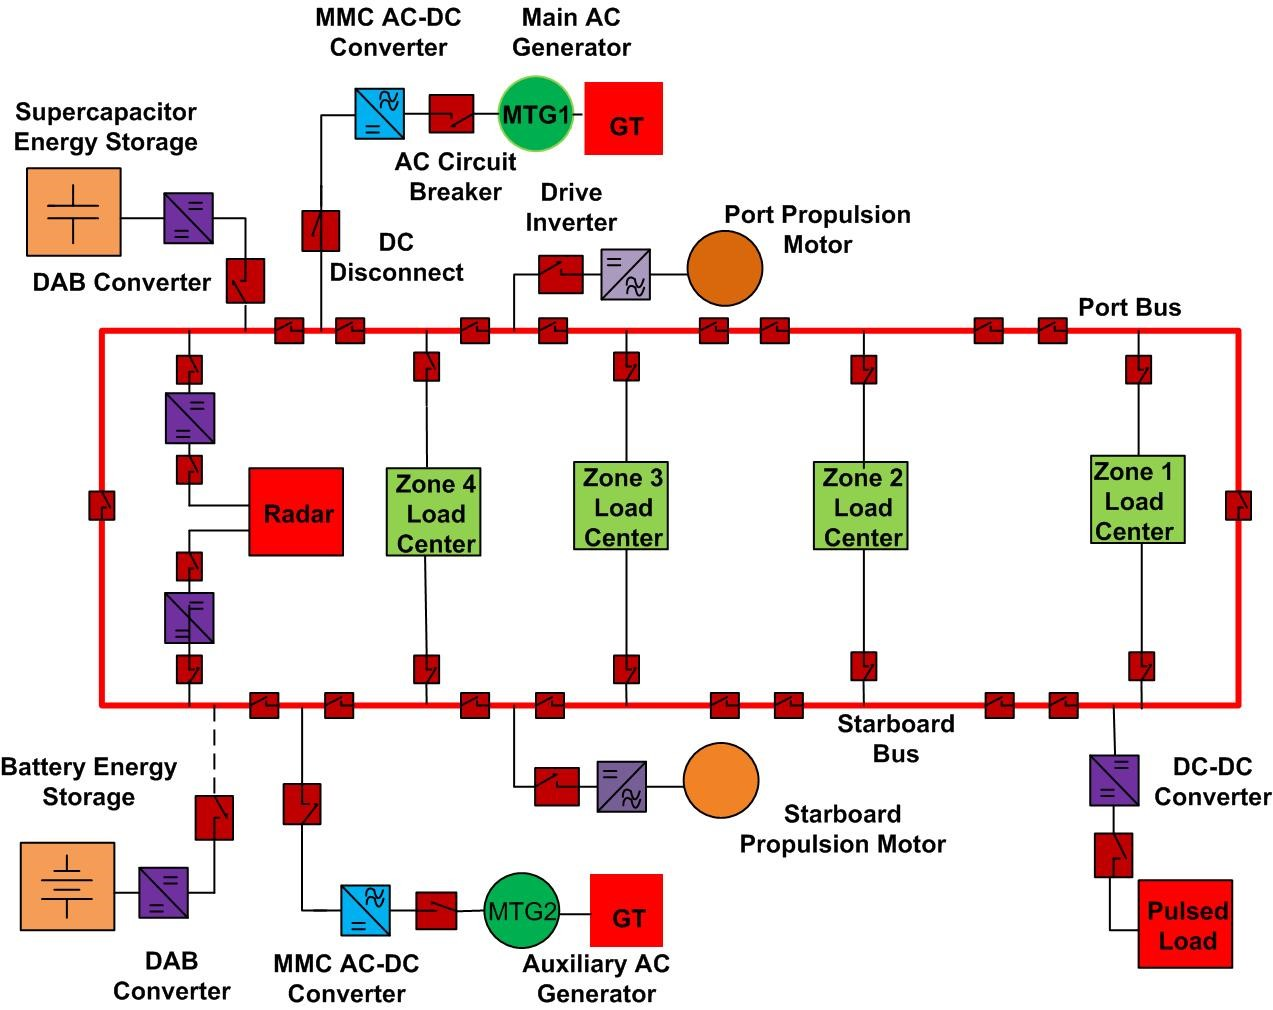
\includegraphics[width=\columnwidth]{f1}
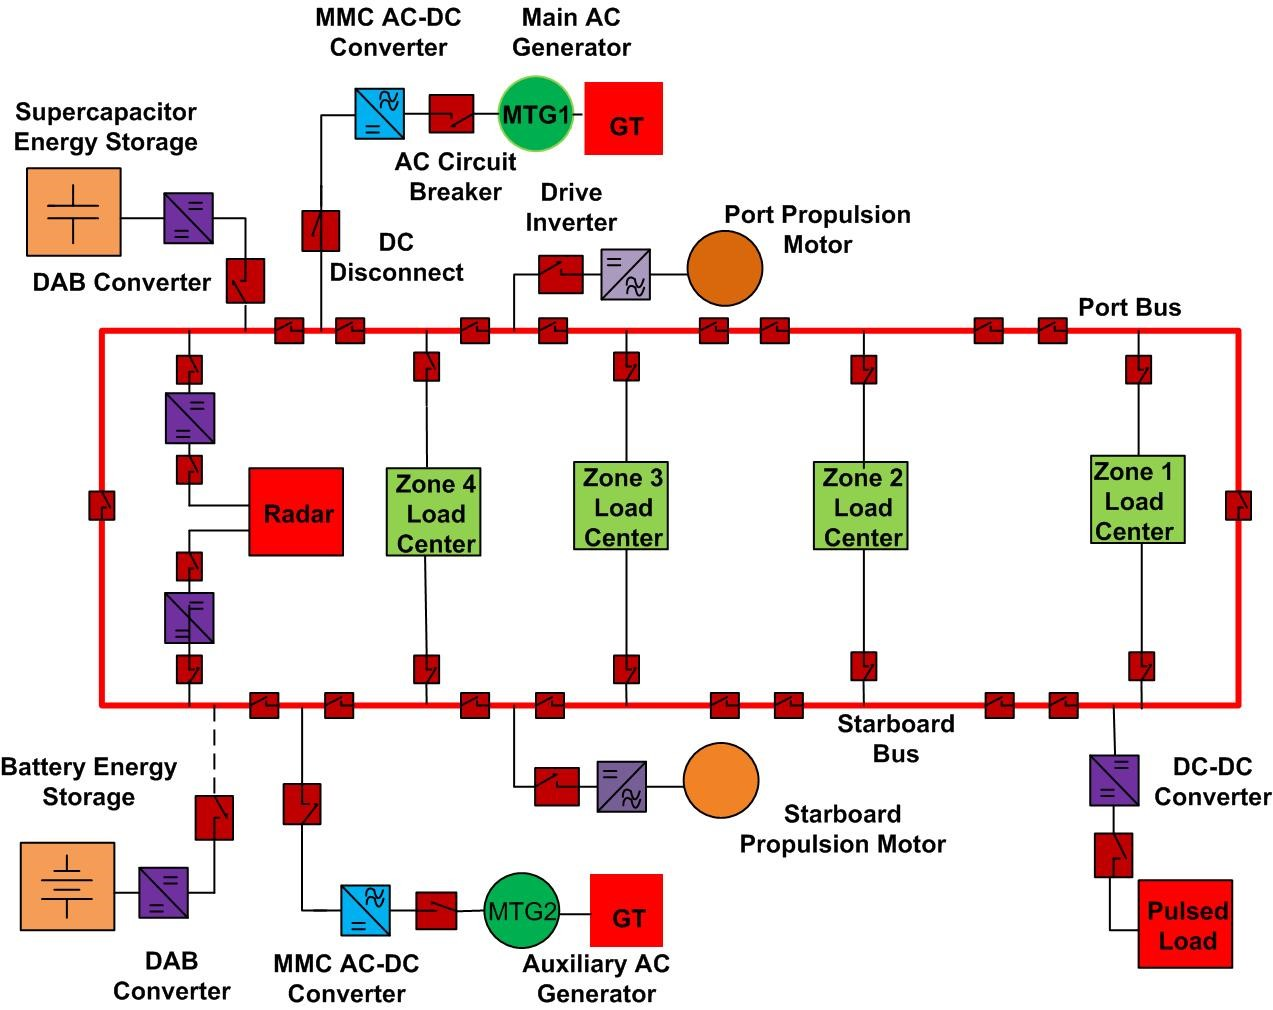
\includegraphics[width=3.46in, height=2.8in]{f1}
\caption{The 5kV MVDC system (40MW).}
\label{sec2_f1}
\end{figure}
%\vspace{-0.27in}
\section{FL Based ESM System Design}
Fig. \ref{sec3_f2} shows a 5kV MVDC system with a FL based ESM system for controlling operation of the HESS. The detailed modeling of the designed FL based ESM system is discussed in \cite{khan2017fuzzy}. In this section, the design steps of FL based ESM system are discussed briefly.
\begin{figure}[ht!]
\centering
%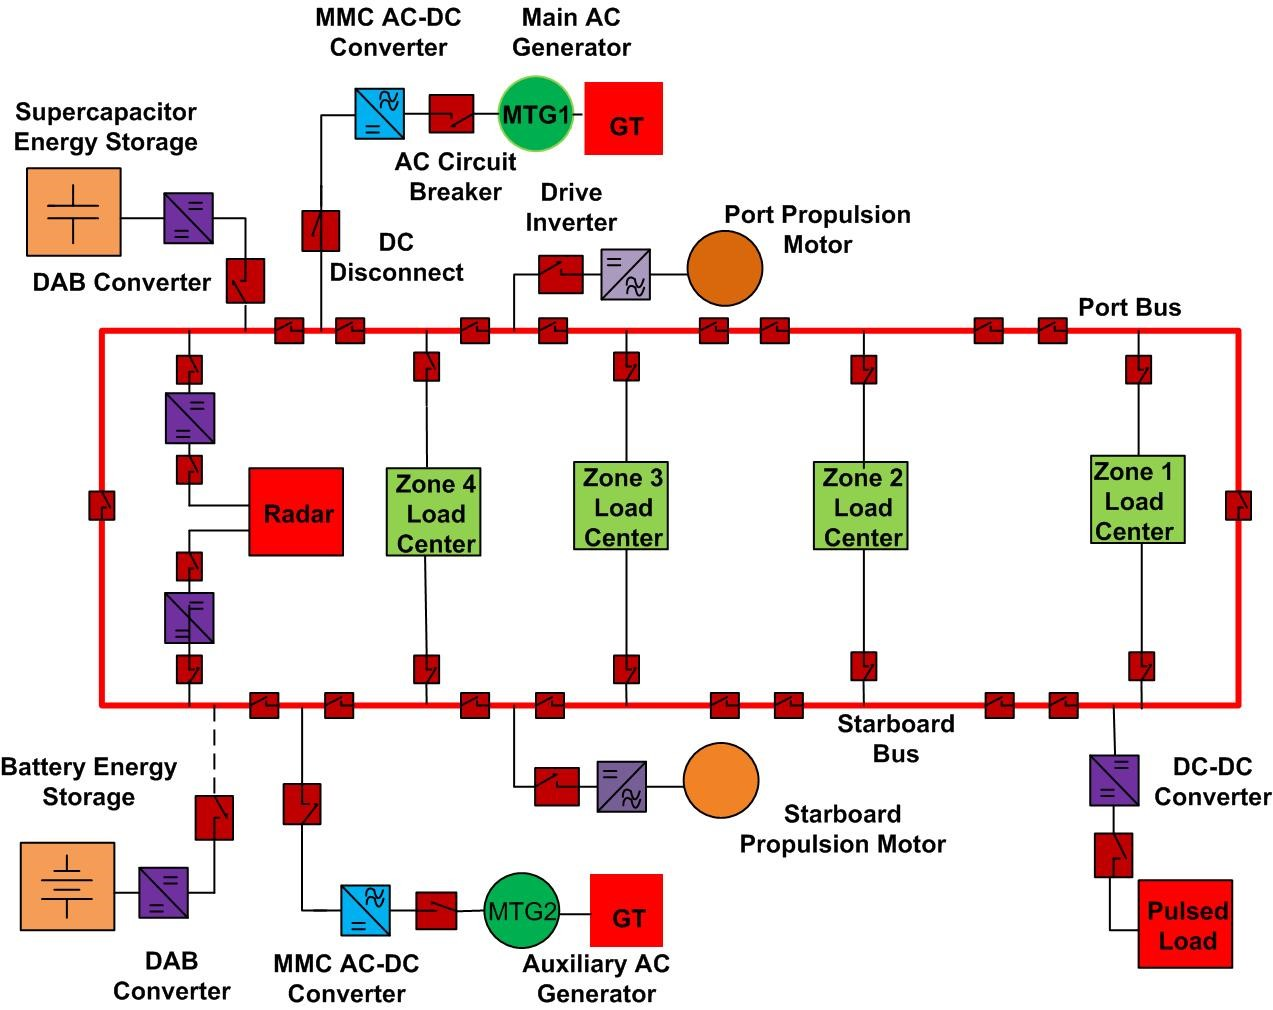
\includegraphics[width=\columnwidth]{f1}
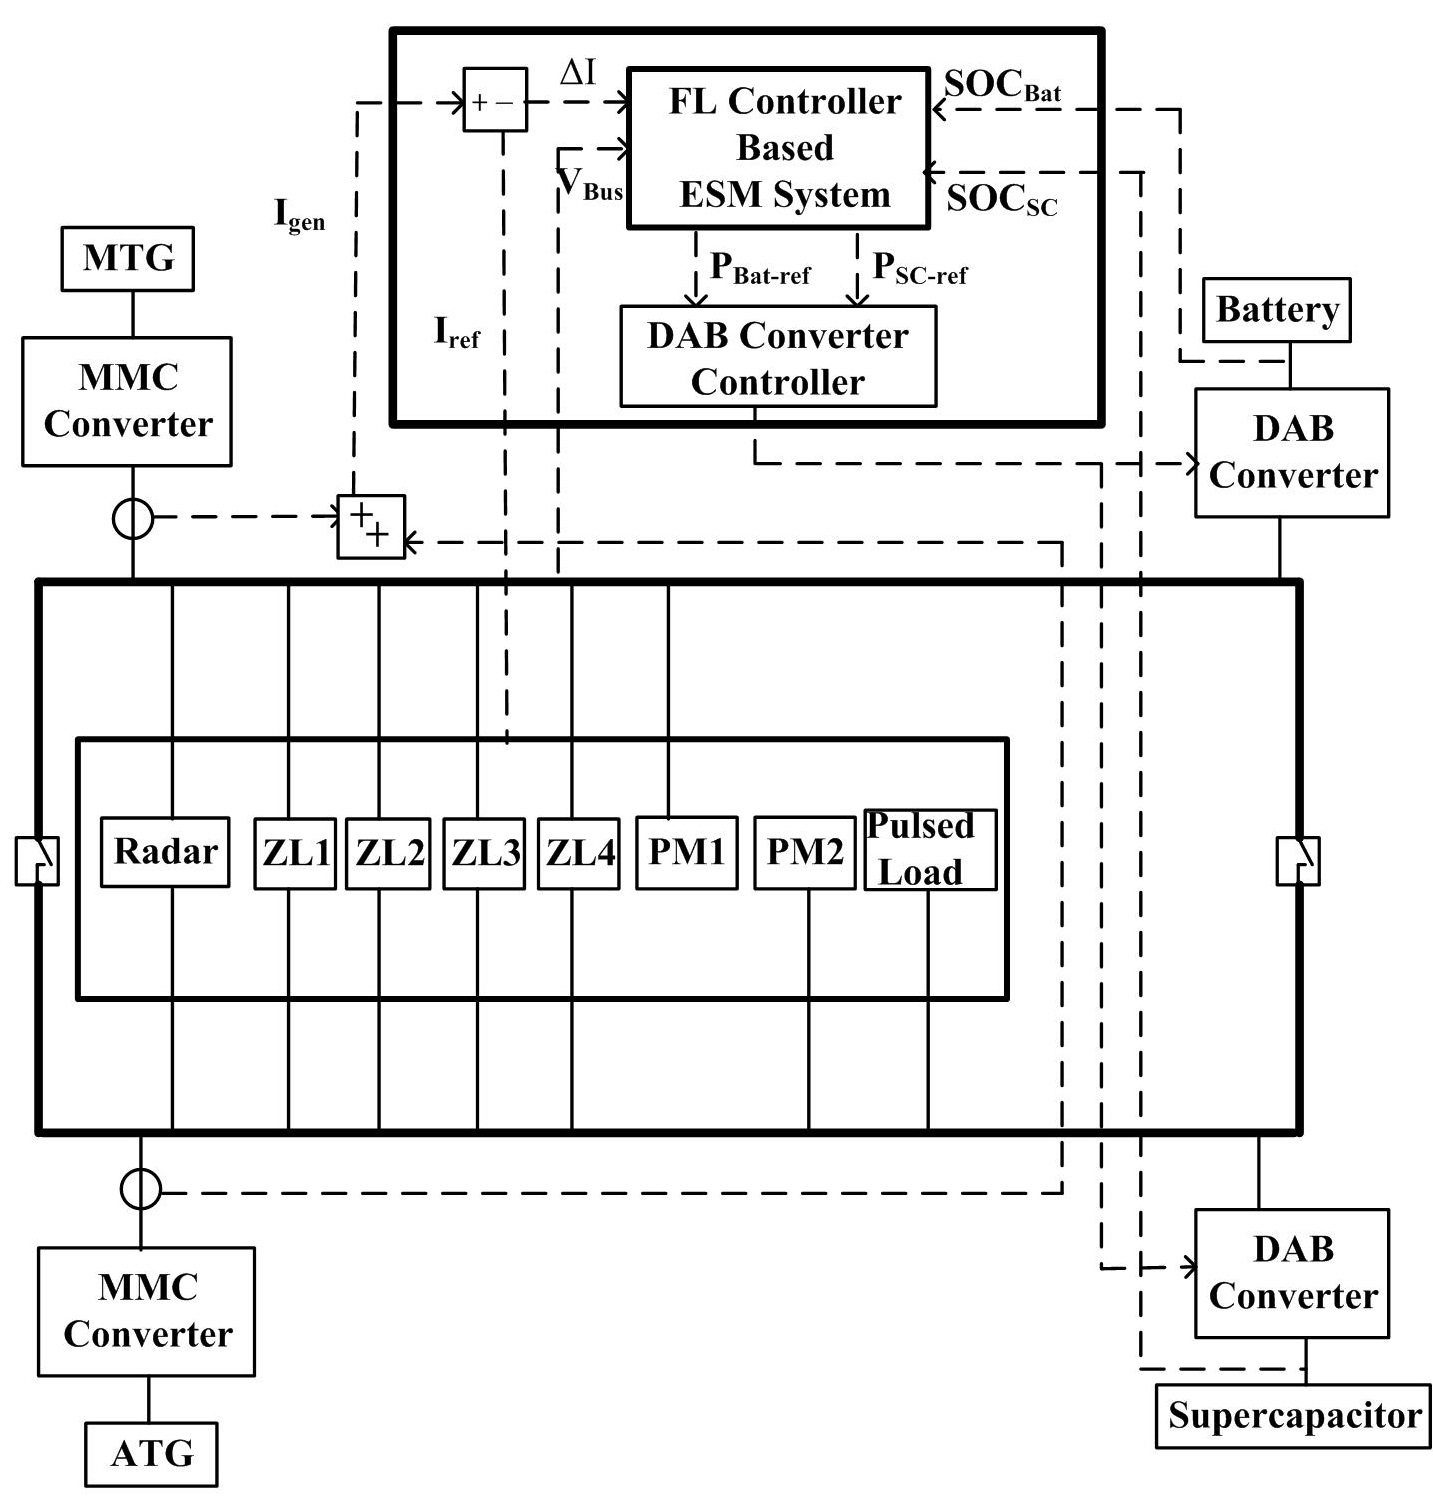
\includegraphics[width=3.51in, height=3.8in]{f2}
\caption{The MVDC system with the FL controller based ESM system.}
\label{sec3_f2}
\end{figure} 

Fig. \ref{sec3_f3} shows the block diagram of the ESM system which has two main steps. In the first step, the total storage reference power ($P_{stor-ref}$) is determined by using the FL controller. Where, $P_{stor-ref}$ represents total charging or discharging power of the battery and supercapacitor combined. After the first step, there is a generation limit checking controller to ensure that the sum of the power demand of the loads and charging reference power of the HESS is within the generation limit (40MW). After passing the $P_{stor-ref}$ through the generation limit checking controller, the aim is to divide $P_{stor-ref}$ between the assigned energy storages as the battery reference power ($P_{Bat-ref}$) and the supercapacitor reference power ($P_{SC-ref}$). To do this, the $P_{stor-ref}$ is passed through a low pass filter (LPF) which separates the respective power for each of them.
\begin{figure}[ht!]
\centering
%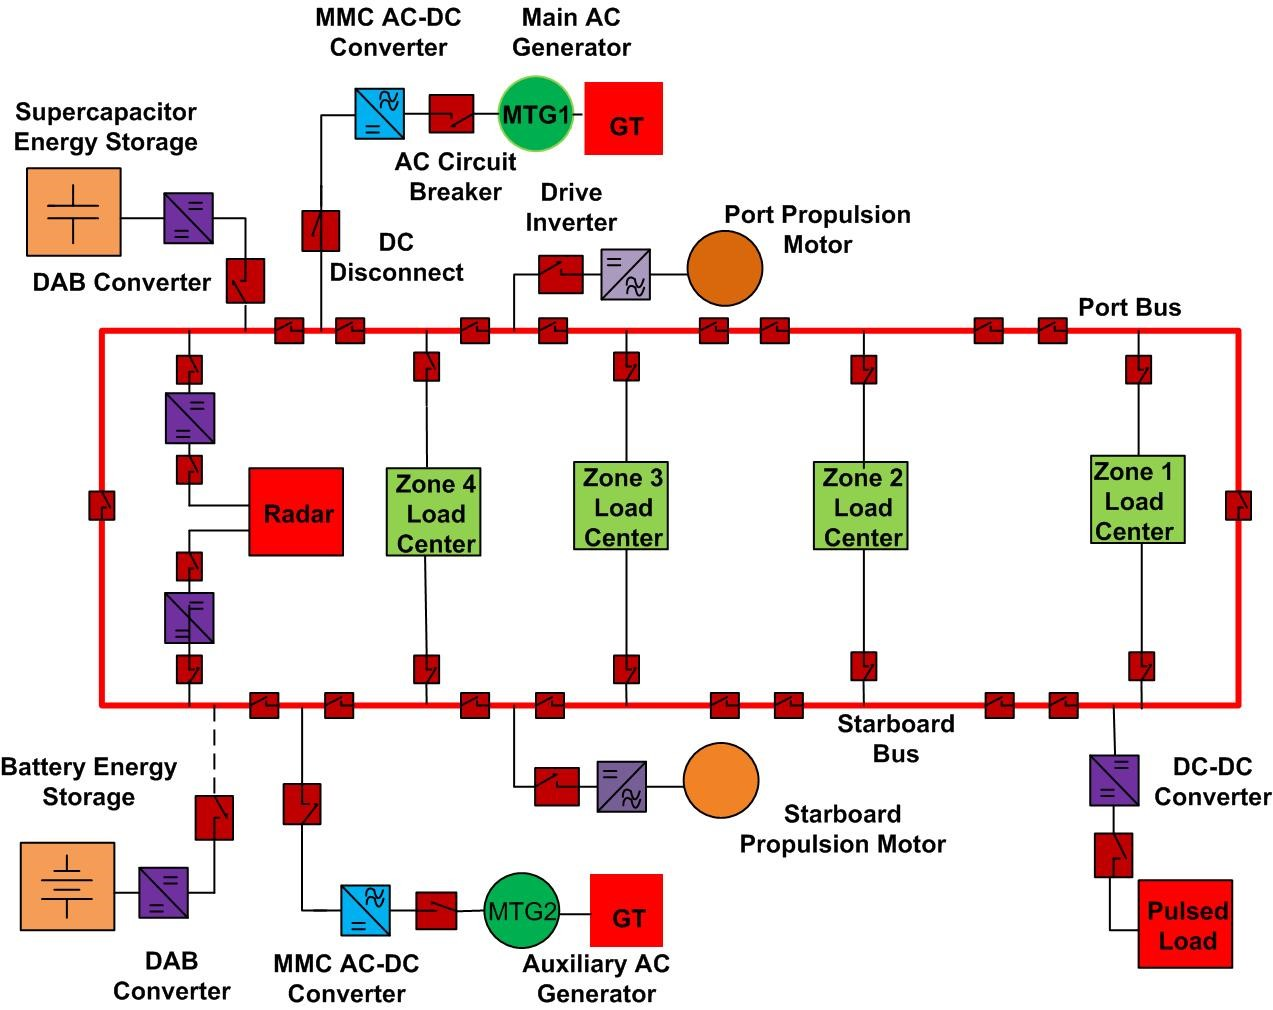
\includegraphics[width=\columnwidth]{f1}
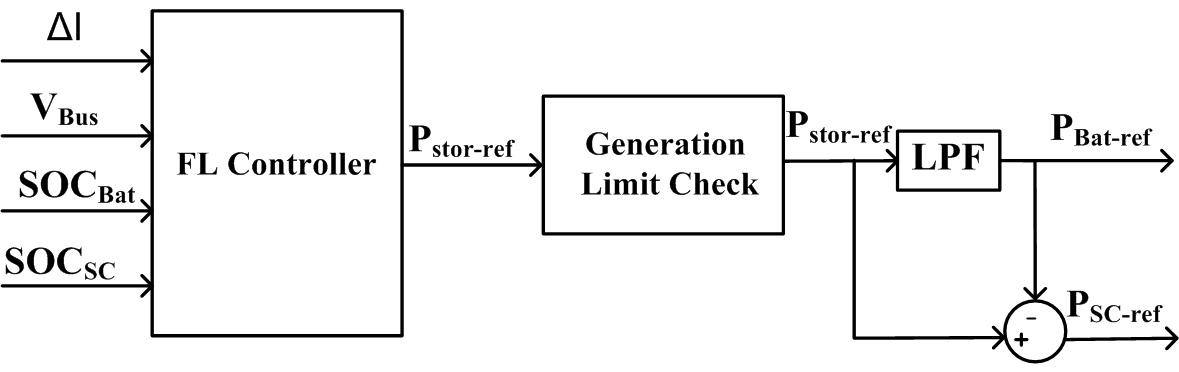
\includegraphics[width=3.46in, height=1.19in]{f3}
\caption{FL controller and LPF based ESM system.}
\label{sec3_f3}
\end{figure}
\subsection{Estimation of $P_{stor-ref}$}
The intention of using FL controller in the first step is to generate the total charging or discharging power of the energy storages based on the condition of the mismatch of the measured load power and actual demanded power and the mismatch of the reference bus voltage of the MVDC system (5kV) and the measured bus voltage. It is also needed to keep the SOC of the energy storages within the limit to avoid the danger of deep discharging and overcharging. Considering these objectives, four input variables based FL controller is designed. The input variables are: $\Delta I$, $V_{Bus}$, $SOC_{Bat}$, and $SOC_{SC}$. Where, $\Delta I$ means the difference between the total reference current ($I_{ref}$) and  the total generated current ($I_{gen}$), $V_{Bus}$ means measured MVDC bus voltage, $SOC_{SC}$ and $SOC_{Bat}$ mean the measured SOC of the supercapacitor and the battery respectively. The output variable is $P_{stor-ref}$ which is the total reference power of the energy storages. The three steps of FL based control technique are discussed here. 

\subsubsection{Fuzzyfication}
\begin{figure}[ht!]
\centering
%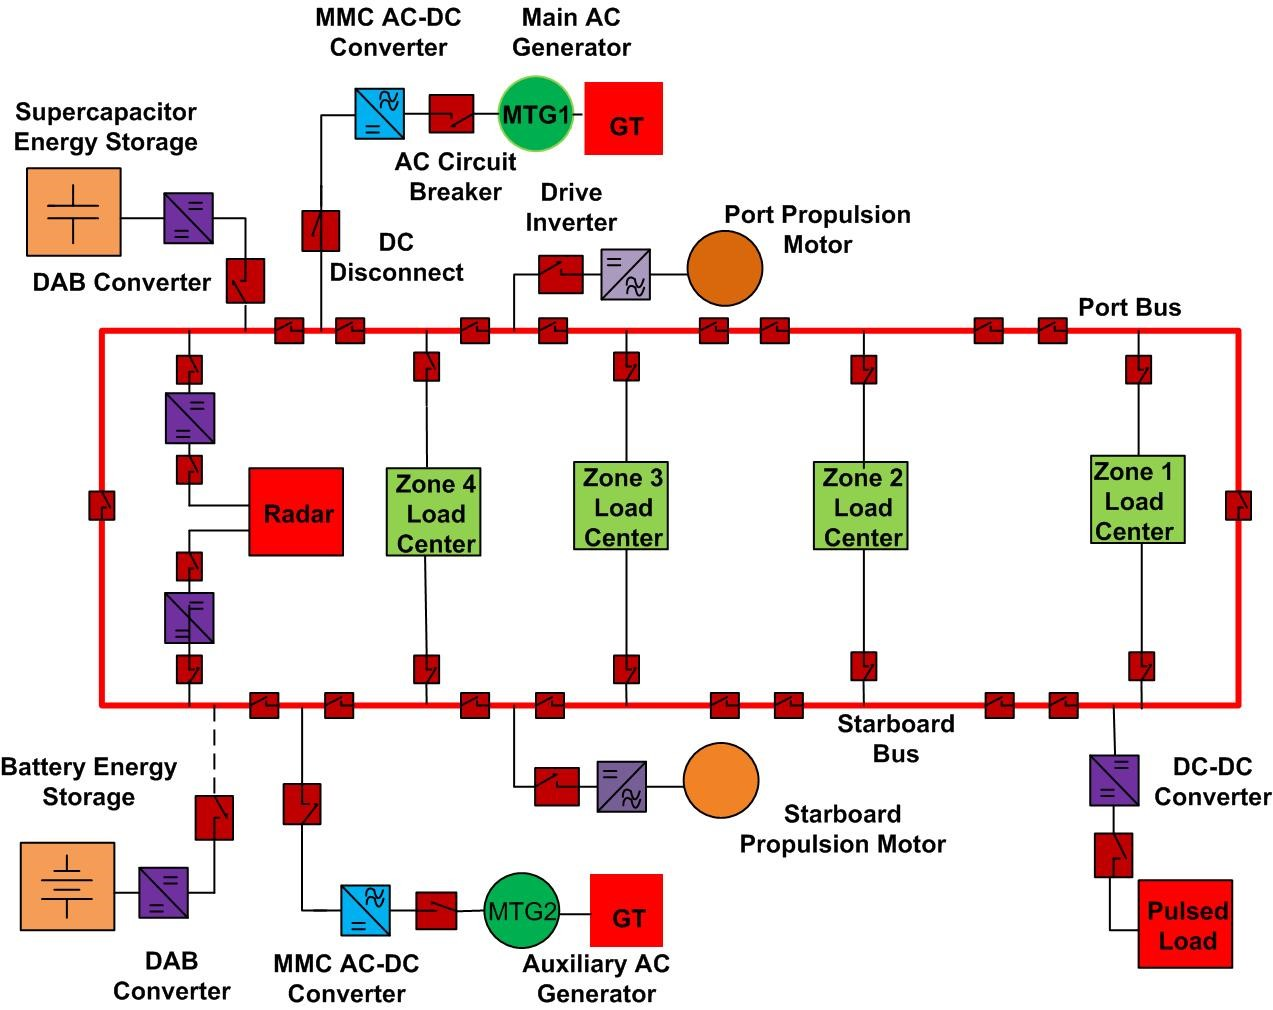
\includegraphics[width=\columnwidth]{f1}
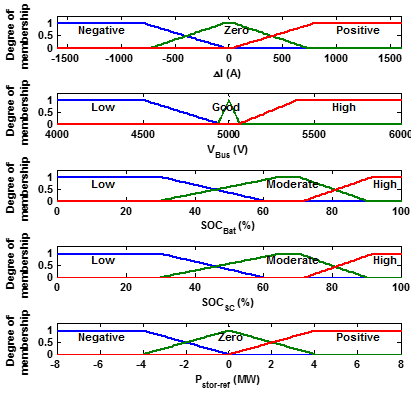
\includegraphics[width=3.46in, height=3.64in]{f4}
\caption{Input and output variables membership functions for the FL controller.}
\label{sec3_f4}
\end{figure}
Fig. \ref{sec3_f4} shows the input and output variables membership functions of the designed FL controller. The operating range of the first input variables, $\Delta I$ is divided into three membership functions, Positive, Negative and Zero. All the membership functions are trapezoidal shaped. The upper and lower limit of the input variable, $\Delta I$ are 1600A and -1600A, respectively. The limits are determined based on the maximum mismatch of the total measured power and total demanded power, the capacity of the energy storages. The second input variable, $V_{Bus}$ also has three membership functions, Low, Good, and High where the Low and High membership functions are the trapezoidal shape and Good membership function is a triangular shape. The upper limit and lower limit of $V_{Bus}$ are  6kV and 4kV, respectively. The third and fourth input variables ($SOC_{Bat}$ and $SOC_{SC}$) have three membership functions where all the membership functions are the trapezoidal shape. The upper limit and lower limit of the third and fourth input variables are 100\% and 0\%, respectively. The output variable, $P_{stor-ref}$ has three membership functions, Positive, Negative and Zero where the Positive and Negative membership functions are the trapezoidal shape and the Zero membership function is a triangular shape.
\subsubsection{Inference} 
The designed FL controller has four input variables and one output variable and each variable has 3 membership functions. Total 81 fuzzy rules are designed to estimate the output variable, $P_{stor-ref}$. As the designed FL controller is associated with five variables and a 2-D table is not sufficient to explain all the fuzzy rules, the fuzzy rules are shown in Table \ref{fl1 controller table}. In the Table \ref{fl1 controller table}, the meaning of the symbols are  N = Negative, Z = Zero, P = Positive, L = Low, G = Good, H = High, and M = Moderate. For example, the first fuzzy rule is: 
\begin{itemize}
\item {\textbf{IF}} $\Delta I$ is N (Negative) {\textbf{AND}} $V_{Bus}$ is L (Low) {\textbf{AND}}  $SOC_{Bat}$ is L (Low) {\textbf{AND}} $SOC_{SC}$ is L (Low), {\textbf{THEN}} $P_{stor-ref}$ is Z (Zero)
\end{itemize}
%table 
\begin{table}[ht!]
%\centering
\processtable{Fuzzy Rules: $P_{stor-ref}$\label{fl1 controller table}}
{\begin{tabu}{p{4.1cm}|p{0.45cm}|p{0.45cm}|[2pt]p{0.45cm}|p{0.45cm}|p{0.45cm}}
\hline
{} &\multicolumn{2}{c|}{\multirow{2}{*}{$\bf P_{stor-ref}$}} & \multicolumn{3}{c}{$\Delta I$} \\
\cmidrule{4-6} 
{}&\multicolumn{2}{c|}{} & N& Z& P\\
\cmidrule{2-6}
\cmidrule{4-6}\tabucline[2pt]{4-6}
{When}&\multirow{3}{*}{$V_{Bus}$} & L& \bf Z & \bf Z & \bf P\\ 
\cmidrule{3-6}
{$SOC_{Bat}$=L AND $SOC_{SC}$=L}&{}& G & \bf Z& \bf Z & \bf P \\ 
\cmidrule{3-6}
&{}& H & \bf Z& \bf Z & \bf P \\
\hline\tabucline[2pt]{4-6}
{When} &\multicolumn{2}{c|}{\multirow{2}{*}{$\bf P_{stor-ref}$}} & \multicolumn{3}{c}{$\Delta I$} \\
\cmidrule{4-6} 
{$SOC_{Bat}$ =L AND $SOC_{SC}$=M/H,}&\multicolumn{2}{c|}{} & N& Z& P\\
\cmidrule{2-6}\tabucline[2pt]{4-6}
{$SOC_{Bat}$=M/H AND $SOC_{SC}$=L,}&\multirow{3}{*}{$V_{Bus}$} & L& \bf N & \bf N & \bf P\\ 
\cmidrule{3-6}
{$SOC_{Bat}$=M AND $SOC_{SC}$=M}&{}& G & \bf N& \bf Z & \bf P \\ 
\cmidrule{3-6}
{}&{}& H & \bf N& \bf Z & \bf P \\
\hline\tabucline[2pt]{4-6}
{ } &\multicolumn{2}{c|}{\multirow{2}{*}{$\bf P_{stor-ref}$}} & \multicolumn{3}{c}{$\Delta I$} \\
\cmidrule{4-6} 
{When}&\multicolumn{2}{c|}{} & N& Z& P\\
\cmidrule{2-6}\tabucline[2pt]{4-6}
{$SOC_{Bat}$=H AND $SOC_{SC}$=M,}&\multirow{3}{*}{$V_{Bus}$} & L& \bf N & \bf N & \bf Z\\ 
\cmidrule{3-6}
{$SOC_{Bat}$=M AND $SOC_{SC}$=H}&{}& G & \bf N& \bf Z & \bf P \\ 
\cmidrule{3-6}
{}&{}& H & \bf N& \bf Z & \bf P \\
\hline\tabucline[2pt]{4-6}
{} &\multicolumn{2}{c|}{\multirow{2}{*}{$\bf P_{stor-ref}$}} & \multicolumn{3}{c}{$\Delta I$} \\
\cmidrule{4-6} 
{}&\multicolumn{2}{c|}{} & N& Z& P\\
\cmidrule{2-6} \tabucline[2pt]{4-6}
{When}&\multirow{3}{*}{$V_{Bus}$} & L& \bf N & \bf N & \bf Z\\ 
\cmidrule{3-6}
{$SOC_{Bat}$=H AND $SOC_{SC}$=H}&{}& G & \bf N& \bf Z & \bf Z \\ 
\cmidrule{3-6}
&{}& H & \bf N& \bf Z & \bf Z \\
\hline\tabucline[2pt]{4-6}

\end{tabu}}{}
\end{table}
\subsubsection{Defuzzyfication}
Fig. \ref{sec3_f4} and Fig. \ref{sec3_f5} show the membership functions of the output variable, $P_{stor-ref}$ and the surface plot for the FL controller, respectively.  Fig. \ref{sec3_f5} shows the response of $P_{stor-ref}$ versus $\Delta I$ and $V_{Bus}$ when $SOC_{Bat}$ and $SOC_{SC}$ are set to 75\% and 82.65\%, respectively.
\begin{figure}[ht!]
\centering
%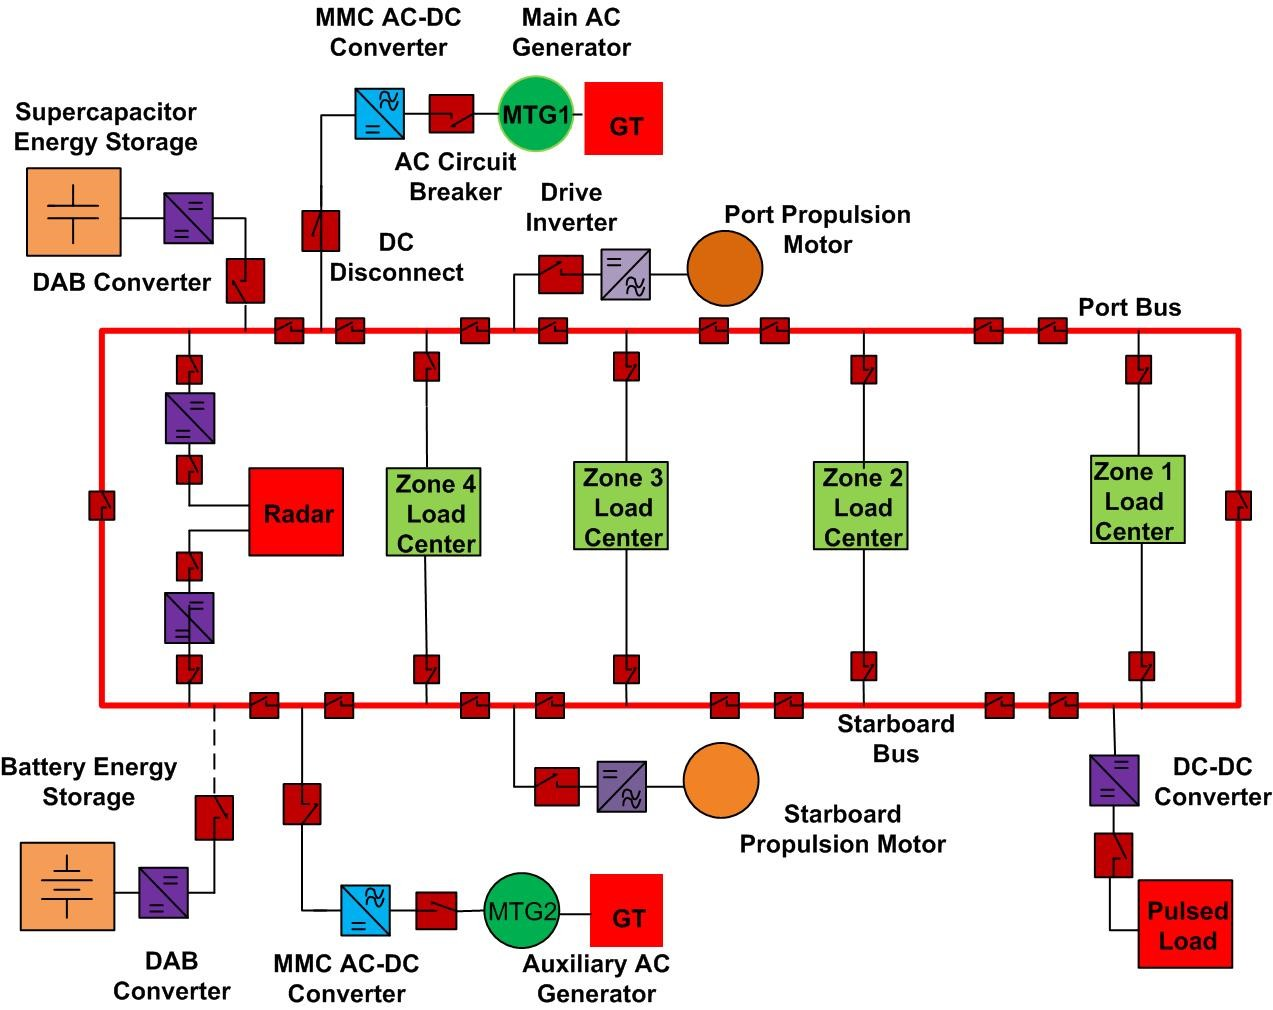
\includegraphics[width=\columnwidth]{f1}
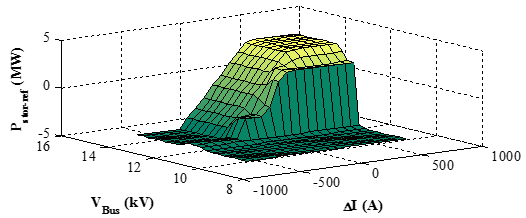
\includegraphics[width=3.46in, height=1.5in]{f5}
\caption{Generated surface of FL controller for $P_{stor-ref}$ versus $\Delta I$, and $V_{Bus}$ when $SOC_{Bat}$, and $SOC_{SC}$ are set to 75\% and 82.65\%, respectively.} 
\label{sec3_f5}
\end{figure} 
\subsection{Estimation of $P_{Bat-ref}$ and $P_{SC-ref}$}
In the second step the $P_{stor-ref}$ is passed through a LPF. The output of the LPF is a low frequency component of $P_{stor-ref}$ which is assigned as the battery reference power, $P_{Bat-ref}$. The difference of $P_{stor-ref}$ and $P_{Bat-ref}$ is the high frequency component of $P_{stor-ref}$ which is assigned as  $P_{SC-ref}$. The transfer function of the LPF is given in (\ref{equation-1}), where $f_{cf}$ is the LPF’s cutoff frequency. As the average models of the converters' are used, the value of cutoff frequency ($f_{cf}$) is set as 1Hz.  
\begin{equation} \label{equation-1}
G_f=\frac {2\pi f_{cf}}{s+2\pi f_{cf}}
\end{equation}

\section{Controller Hardware-in-the-Loop (CHIL) Based Test System}
\subsection{Implementation of Fuzzy Logic Controller on FPGA System}
During the offline simulation and the initial real-time simulation cases, the fuzzy logic controller is designed using the MathWorks fuzzy logic toolbox \cite{WinNT6}. But to implement the FL controller in FPGA, VHDL (Very high speed integrated circuit Hardware Description Language) code is used as the Matlab HDL (Hardware description language) coder does not generate the automatic VHDL code for the fuzzy logic controller, the FL controller is designed from teh scratch. The FL controller has three major parts: 1) Fuzzification, 2) Inference and 3) Defuzzification.

\subsubsection{Fuzzification}
In this part, the membership functions of the input and output variables are defined. The membership function shapes are typically triangular, trapezoidal, Gaussian, and bell shaped. Fuzzy crisp input values are converted into membership values in the interval [0 1]. In fuzzification, the degree of membership is determined by locating the input in the membership function. The designed FL controller has four input variables ($\Delta I$, $V_{Bus}$, $SOC_{Bat}$, and $SOC_{SC}$) and one output variable ($P_{stor-ref}$). The membership functions of the input and output variables are shown in Fig. \ref{sec3_f4}. The first input variables, $\Delta I$ has three membership functions (Positive, Negative, Zero) and all of them are trapezoidal shaped. Fig. \ref{sec4_f6} shows a trapezoidal shaped membership function. The trapezoidal shaped membership function is divided into five regions. As a function of x, the five regions of the trapezoidal shaped membership function is represented in (\ref{equation-2}). Where x represents the crisp values of the input variables, y represents the degree of membership ($\mu$) and $a$, $b$, $c$, $d$ are four scalar parameters which define the shape of the trapezoidal membership function \cite{anand2012design}.
\begin{figure}[ht!]
\centering
%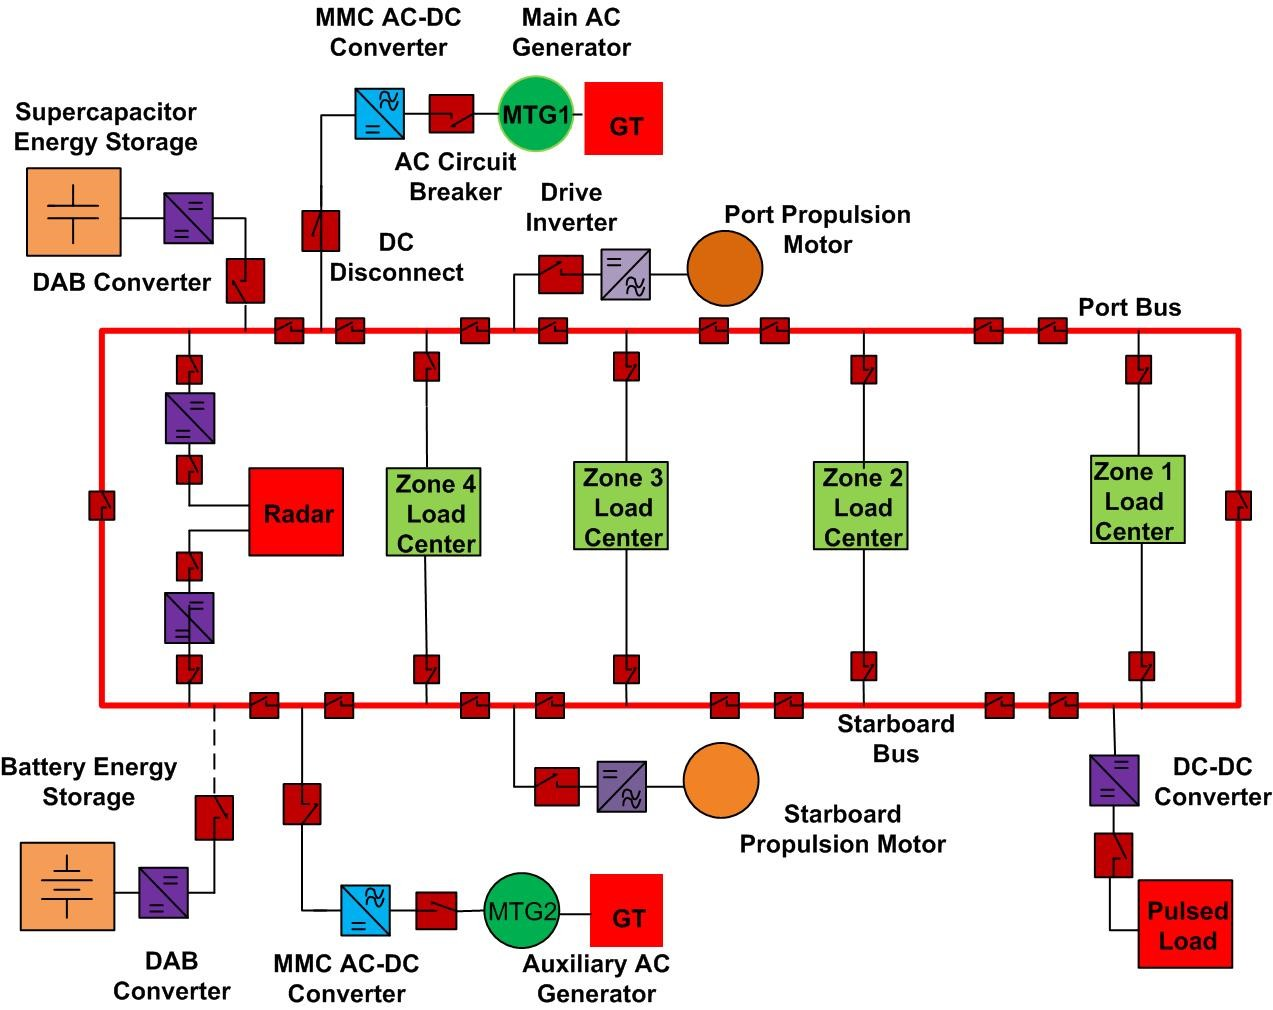
\includegraphics[width=\columnwidth]{f1}
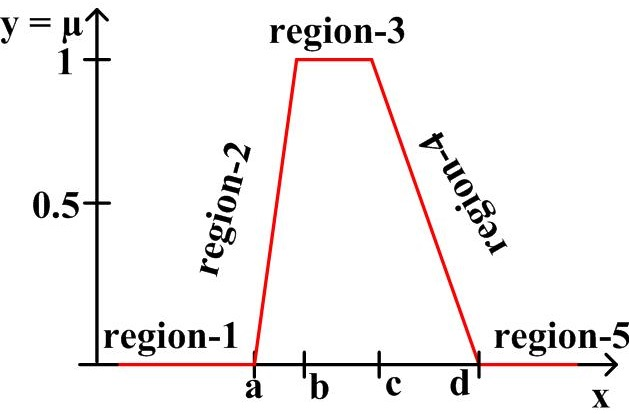
\includegraphics[width=2.0in, height=1.3in]{f6}
\caption{Trapezoidal-shaped membership functions.}
\label{sec4_f6}
\end{figure} 
\begin{equation}\label{equation-2}
f(x;a,b,c,d)=
    \begin{cases}
      0, &  x\leq a\\
      \frac{x-a}{b-a}, & a\leq x \leq b \\
       1, & b\leq x \leq c \\
       \frac{d-x}{d-c}, & c\leq x \leq d \\
       0, &  d\leq x
    \end{cases}
\end{equation}
For example, the Zero membership function of $\Delta I$ is represented in (\ref{equation-3}) where the values are $a$ = -720, $b$ = -40, $c$ = 40, and $d$ = 720. Similarly the other two membership functions (Negative and Positive) are represented. 

\begin{equation}\label{equation-3}
f(x;a,b,c,d)=
    \begin{cases}
      0, &  x\leq -720\\
      \frac{x-(-720)}{(-40)-(-720)}, & -720\leq x \leq -40 \\
       1, & -40\leq x \leq 40 \\
       \frac{720-x}{720-40}, & 40\leq x \leq 720 \\
       0, &  720\leq x
    \end{cases}
\end{equation}
The second input variables, $V_{Bus}$ has three membership functions (High, Low and Good). The Low and High membership function are trapezoidal shaped and they are designed as the similar way shown for the input variable $\Delta I$. The Good membership function is triangular shaped and it is divided into four regions. Fig. \ref{sec4_f7} shows a triangular shaped membership function. As a function of x, the four regions of the triangular shaped membership function is represented in (\ref{equation-4}). Where x represents the crisp values of the input variables, y represents the degree of membership ($\mu$) and $a$, $b$, and $c$ are three scalar parameters which define the shape of the triangularly shaped membership function. The Good membership function of the input variable, $V_{Bus}$ is triangular shaped, where the values are $a$ = 4940, $b$ = 5000, and $c$ = 5060. The third and fourth input variables ($SOC_{Bat}$, and $SOC_{SC}$) have three trapezoidal shaped membership functions and they are designed as the similar way shown in (\ref{equation-2}). The output variable, $P_{stor-ref}$ has two trapezoidal shaped membership functions (Negative, Positive), they are designed as the similar way shown in (\ref{equation-2}), one triangular shaped membership function (Zero) and it is designed as the similar way as shown in (\ref{equation-4}). 
\begin{figure}[ht!]
\centering
%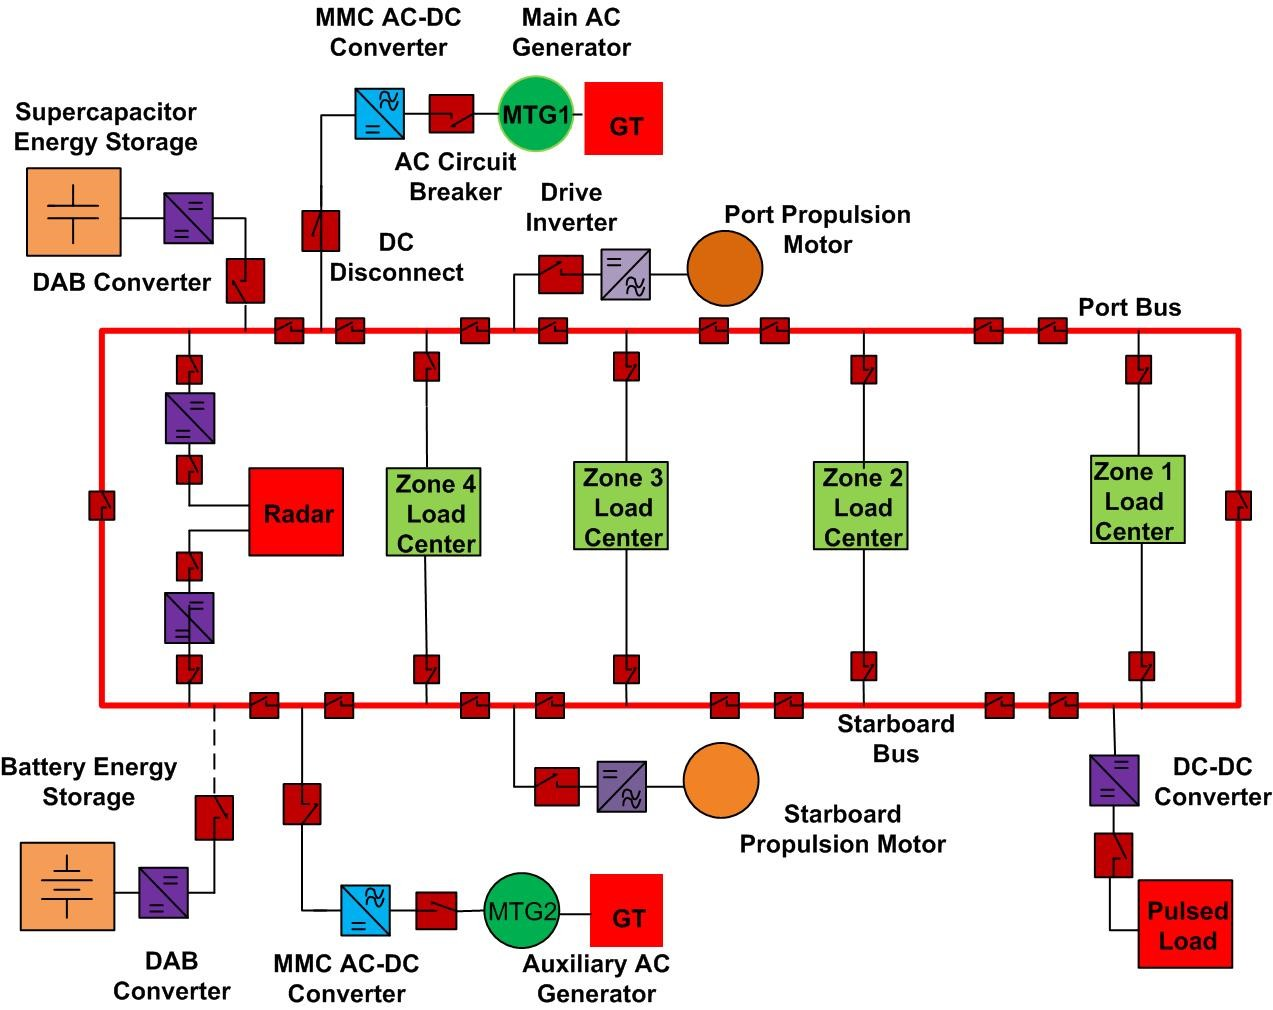
\includegraphics[width=\columnwidth]{f1}
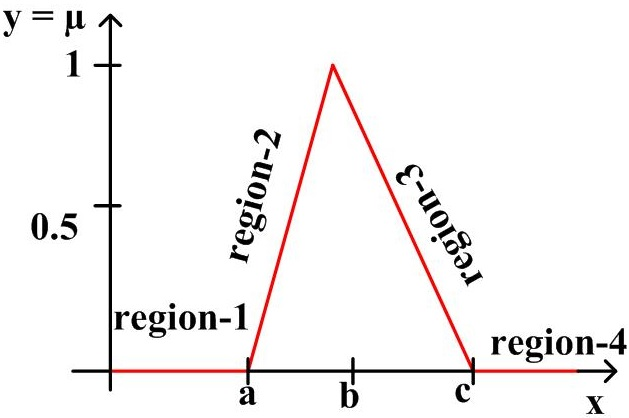
\includegraphics[width=2.0in, height=1.3in]{f7}
\caption{Triangular-shaped membership functions.}
\label{sec4_f7}
\end{figure}
\begin{equation}\label{equation-4}
f(x;a,b,c)=
    \begin{cases}
      0, &  x\leq a\\
      \frac{x-a}{b-a}, & a\leq x \leq b \\
       \frac{c-x}{c-b}, & b\leq x \leq c \\
       0, &  c\leq x
    \end{cases}
\end{equation}
\subsubsection{Inference}Fuzzy rules create the relationship between the output domain fuzzy sets and the input domain fuzzy sets. A fuzzy inference system makes fuzzy decisions based on fuzzy inputs and rules. The two common fuzzy operators for multiples antecedents are “fuzzy intersection or conjunction or minimum (AND)” and “fuzzy union or disjunction or maximum (OR)”. The fuzzy rules are shown in Table I and the first fuzzy rule is written in section III. For example, in a certain moment, the FL controller receives $\Delta I$ = -1000A, $V_{Bus}$ = 4400V, $SOC_{Bat}$ = 20\%, and $SOC_{SC}$ = 25\% as the inputs. After using the designed membership functions for the input variables, the degree of membership ($\mu$) of the input variables are  $\mu_{Negative}(\Delta I) = 1$, $\mu_{Low}(V_{Bus}) = 1$,  $\mu_{Low}(SOC_{Bat}) = 1$, and  $\mu_{Low}(SOC_{SC}) = 1$. According to first fuzzy rule, the degree of membership function, Zero of the output variable, $P_{stor-ref}$ is given in (\ref{equation-5})
\begin{multline}\label{equation-5}
\mu_{Zero}(P_{stor-ref})= min[(\mu_{Negative}(\Delta I), \mu_{Low}(V_{Bus}), \\
\mu_{Low}(SOC_{Bat}), \mu_{Low}(SOC_{Bat})]
\end{multline}
\subsubsection{Defuzzification} In defuzzification process, the degree of membership functions ($\mu$) of the output variable ($(P_{stor-ref}$) is converted to the actual crisp value. For defuzzification, the center of sums method is used \cite{ross2009fuzzy}. This method is similar to the weighted average method and it is faster than the many commonly used defuzzification methods. The output defuzzified crisp value ($z^{\ast}$) is calculated by using (\ref{equation-6}).  Here, $C_k(z)$ is the output fuzzy set and  $\bar{z}$ denotes the distance to the centroid of each of the respective membership functions. 
\begin{equation}\label{equation-6}
z^{\ast}=\frac{\sum_{k=1}^{n}\mu C_k(z)\int_z \bar{z} dz}{\sum_{k=1}^{n}\mu C_k(z)\int_z dz}
\end{equation}
\subsubsection{Implementation of CHIL on FPGA}
For CHIL implementation the ‘Xilinx Virtex-7 FPGA VC707 Evaluation Kit’ which is available with the OP7200 FPGA. The fuzzy logic controller has a very wide range of numbers. The degrees of membership need to be kept accurate to at least three decimal places to operate the FL controller properly. The numerator part of (\ref{equation-6}) can be in the range of $1 \times 10^{18}$.To accommodate this huge range with fixed point numbers at least 69 bits are necessary. The Xilinx vartex-7 FPGA running at 100MHz was not able to complete basic 69-bit arithmetic operations within in the allocated time (10ns).  For this reason the IEEE 754 single precision floating point number format \cite{sites2008ieee} is used for all the calculations. The floating point arithmetic functions for the VHDL code are generated using the Xilinx ‘LogiCORE IP Floating-Point Operator v5.0’ product. The rest of the system is designed using system generator, digital signal processor (DSP) provided by Xilinx.

Fig. \ref{sec4_f8} shows the model built with RT-XSG and Xilinx system generator blocks which are used to generate the final bit stream. As seen in the figure the $\Delta I, V_{bus}, SOC_{BAT} and SOC_{SC}$ signals are first converted from double to single precision floating point number  and then sent from the real time simulator to the FPGA running the FL algorithm. The fuzzification process uses the values of the signals sent from the simulator to generate the membership values. Then these values are used in the defuzzification and inference process to generate the power reference needed for the energy storage. The generated power reference is then sent to the simulator and converted back to double precision floating point number and used for the simulation.   
\begin{figure}[ht!]
\centering
%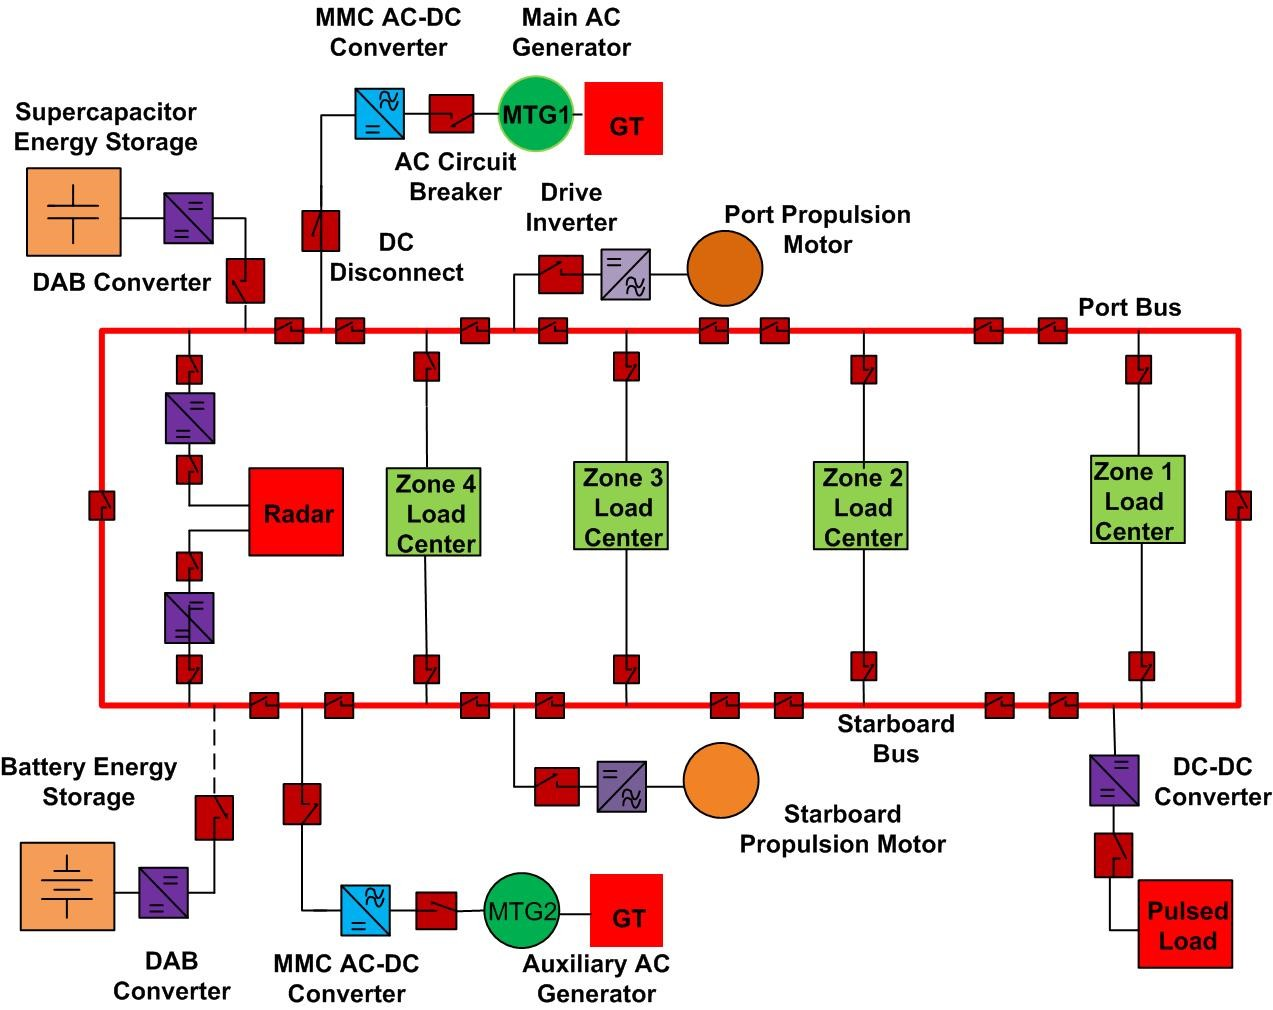
\includegraphics[width=\columnwidth]{f1}
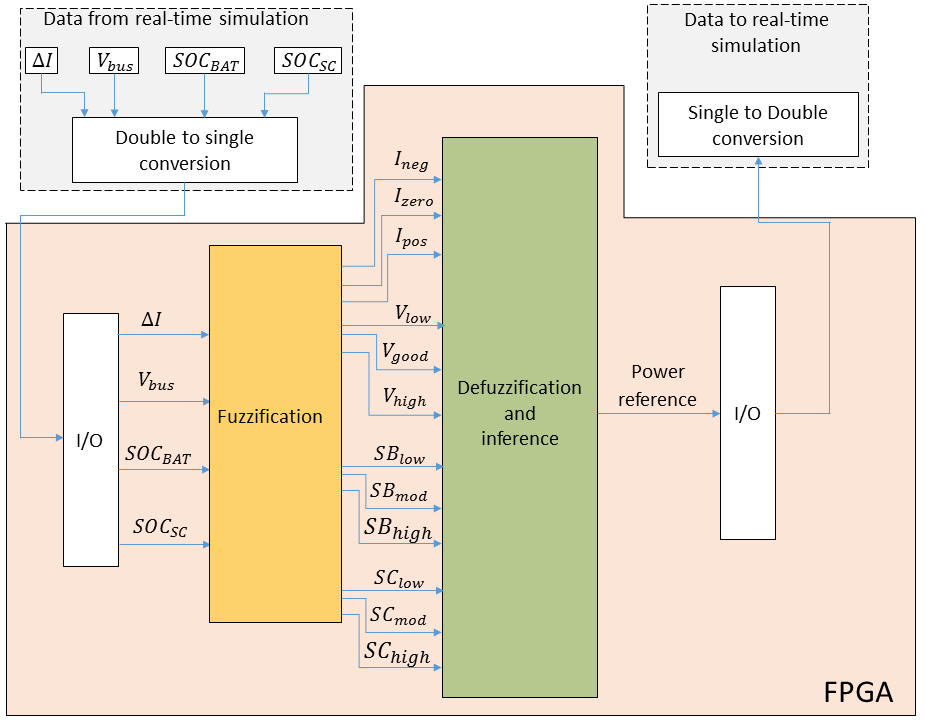
\includegraphics[width=3.5in]{f8}
\caption{Xilinx system generator model.}
\label{sec4_f8}
\end{figure}

Fig. \ref{sec4_f9} shows the implementation of one of the 81 rules derived from Table 1. From Fig. \ref{sec4_f9}, in the black box, the minimum value of all degrees of memberships is determined for a single rule. The output of this part is the $\mu_{Zero}(P_{stor-ref})$ according to (\ref{equation-5}). In the dotted box, the individual numerator ('A') and denominator ('B') component of (\ref{equation-6}) are determined for that respective rule. From Fig. \ref{sec4_f9}, the output ‘A’ represents the individual numerator component of (\ref{equation-6}) and the output ‘B’ represents the individual denominator component of (\ref{equation-6}) for a single rule. Finally, all the numerator ('A') components are summed and all the denominator ('B') components are summed individually for all the rules. Eventually, the sum of numerator components is divided by the sum of the denominator components according to (\ref{equation-6}) to generate the crisp output value ($P_{stor-ref}$). 
\begin{figure}[ht!]
\centering
%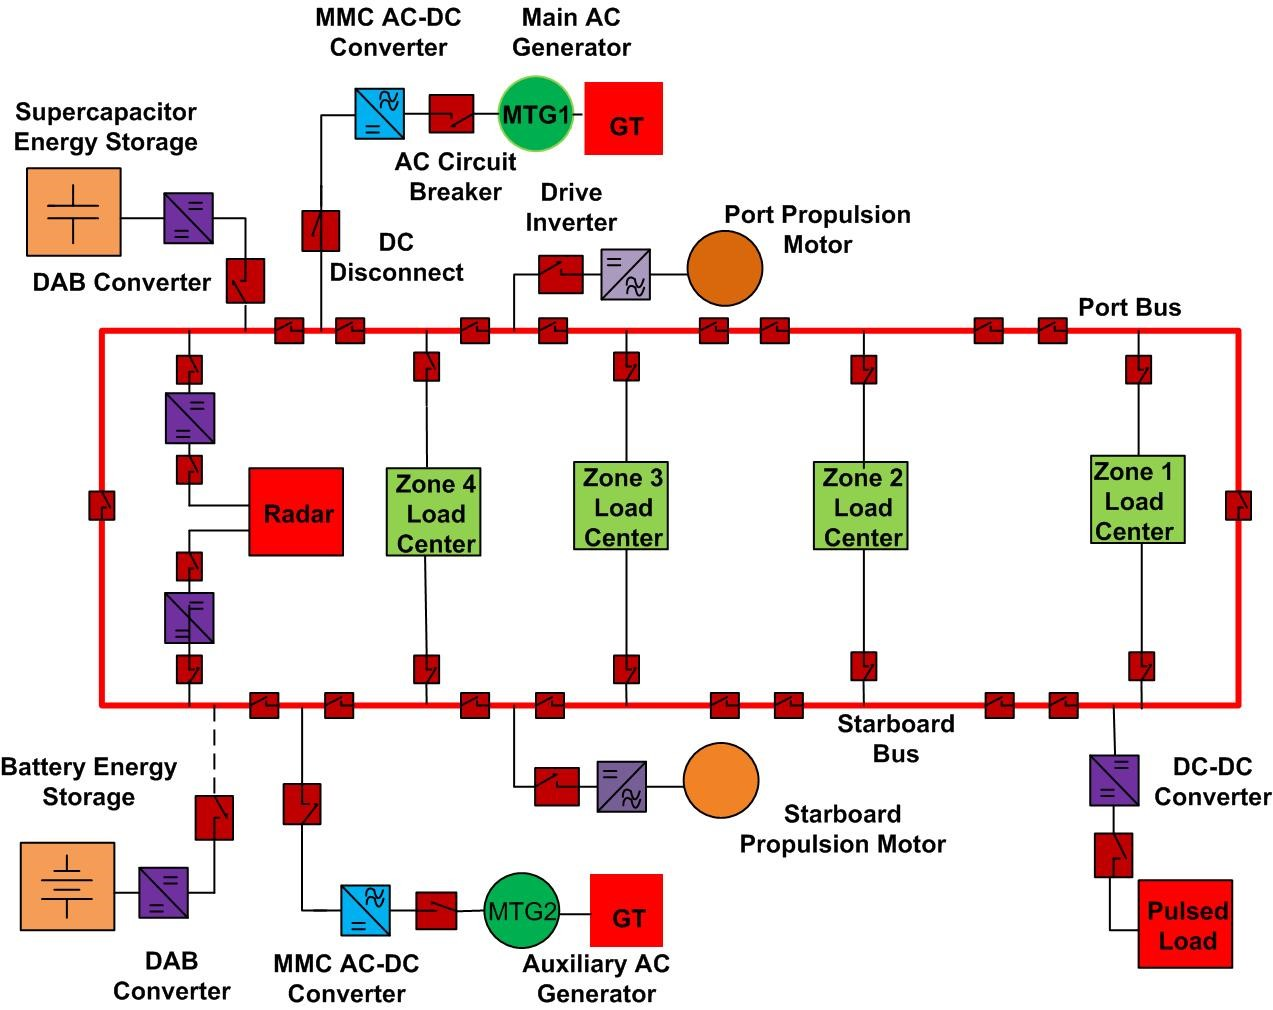
\includegraphics[width=\columnwidth]{f1}
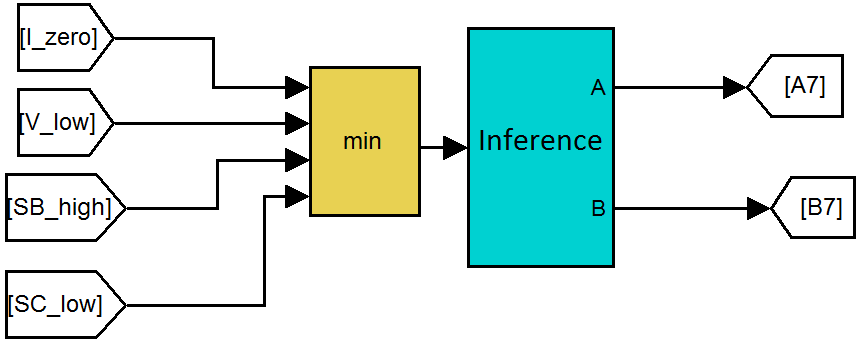
\includegraphics[width=3.5in]{f9}
\caption{Implementation of inference and defuzzification.}
\label{sec4_f9}
\end{figure}

\subsection{CHIL Based Test System Setup}
\subsubsection{Introduction of CHIL Environment}
\paragraph{Digital Real-Time Simulator (DRTS)}
RT-LAB real-time simulator is used for real-time simulation of MVDC power system which uses MATLAB/Simulink platform for modeling the system. The system modeled in Simulink is converted to C code and loaded in DRTS for real-time execution of the system. Both digital and analog inputs and outputs (I/O) interfacing facilities are available with the real-time simulator to communicate with external devices. The Target computer (real-time simulator) uses TCP/IP network to communication with the Host computer. REDHAT real-time operating system is used to run the target computer. RT-LAB uses advanced fixed time-step solvers and computational techniques designed for the real-time simulation which is known as ARTEMIS \cite{mikkili2015review}. 

   
{\textbf{OP7020: }}The OP7020 is an expansion unit for the RT-LAB simulator and it contains a Xilinx Virtex-7 FPGA. To communicate with other FPGA devices (for examples OP7000 and OP5607) or external controllers, it has 16 high-speed fiber optic links using Small Form-factor Pluggable (SFP) transceivers. It follows Aurora (1 to 5 Gbits), Gigabit Ethernet (1 Gbit) protocols. The custom protocol can be also implemented. In order to connect OP7020  with the Target computer (Opal-RT simulator), high speed (30Gbps) fiber-optic X4 links are available \cite{FPGA_EXP}. 


{\textbf{OP5607: }}The OP5607 is a Xilinx Virtex-7 FPGA based I/O expansion unit. It has 8 signal conditioning and analog/digital converter modules with 16 analog and 32 digital channels. Which supports 128 analog and 256 digital signals. To connect with other FPGA devices (OP7020, OP4500, and OP7020) and external controllers, 16 high speed (speed from 1 to 5Gbps) SFP multi-mode fiber optic links are interfaced with OP5607.  It follows Aurora (1 to 5 Gbits), Gigabit Ethernet (1 Gbit), and customer requirements based protocols \cite{FPGA_EXP}. In the front side of the OP5607, there are mini-BNC terminals for monitoring signals through an oscilloscope. It has high speed (30Gbps) PCI Express gen2 x4 fiber-optic links to interface with the Target computer (Opal-RT simulator). 
\subsubsection{CHIL Simulation Interfacing}
Fig. \ref{ch5_f111} shows the block diagram of the CHIL simulation setup. The Host computer (not shown) is an Intel core i7, 3.2GHz processor and it is connected to the Target-real time simulator via Ethernet cable. Four different cores of the real-time simulator are used to load and run four different subsystems of the loads, sources, battery and supercapacitor. The available Xilinx System Generator (XSG) library and RT-XSG are used to model the FL controller based ESM system. RT-XSG library is also used to model analog outputs in OP5607. The RT-XSG is capable of compiling the model and generates VHDL code and FPGA bit streams. The bit stream file of the FL based ESM system controller is implemented in the FPGA board available with OP7020. The OP5607 is used to produce analog output signals by loading the analog output bit stream file in OP5607. The target computer (real-time simulator) is connected to the OP5607 and OP7020 via fiber-optic PIC express links. 


Fig. \ref{ch5_f112} shows the experimental setup for the CHIL based test system. Fig. \ref{ch5_f112a} shows the front panel. Where the top FPGA board, OP7020 is used to implement the FL based ESM controller for CHIL based testing. From Fig. \ref{ch5_f112b}, the bottom board is OP5607 and it is connected to the scope to show the analog output results. The top FPGA board (OP7020) works as a master and bottom FPGA (OP5607) board works as a slave. A black audio cable is used for synchronization between them. There are quick monitoring ports on the front panel of OP5607. The RJ45 connector (white cable) connects analog/digital ports of OP5607 to quick monitoring ports. Eventually, analog output signals are passed from the quick monitoring ports to the oscilloscope through the BNC connectors.  Fig. \ref{ch5_f112b} shows the back panel. From Fig. \ref{ch5_f112b}, the orange cables are fiber optic PCI express cables which connect OP5607 and OP7020 to the real-time simulator. 

\begin{figure}[h!]
\centering
%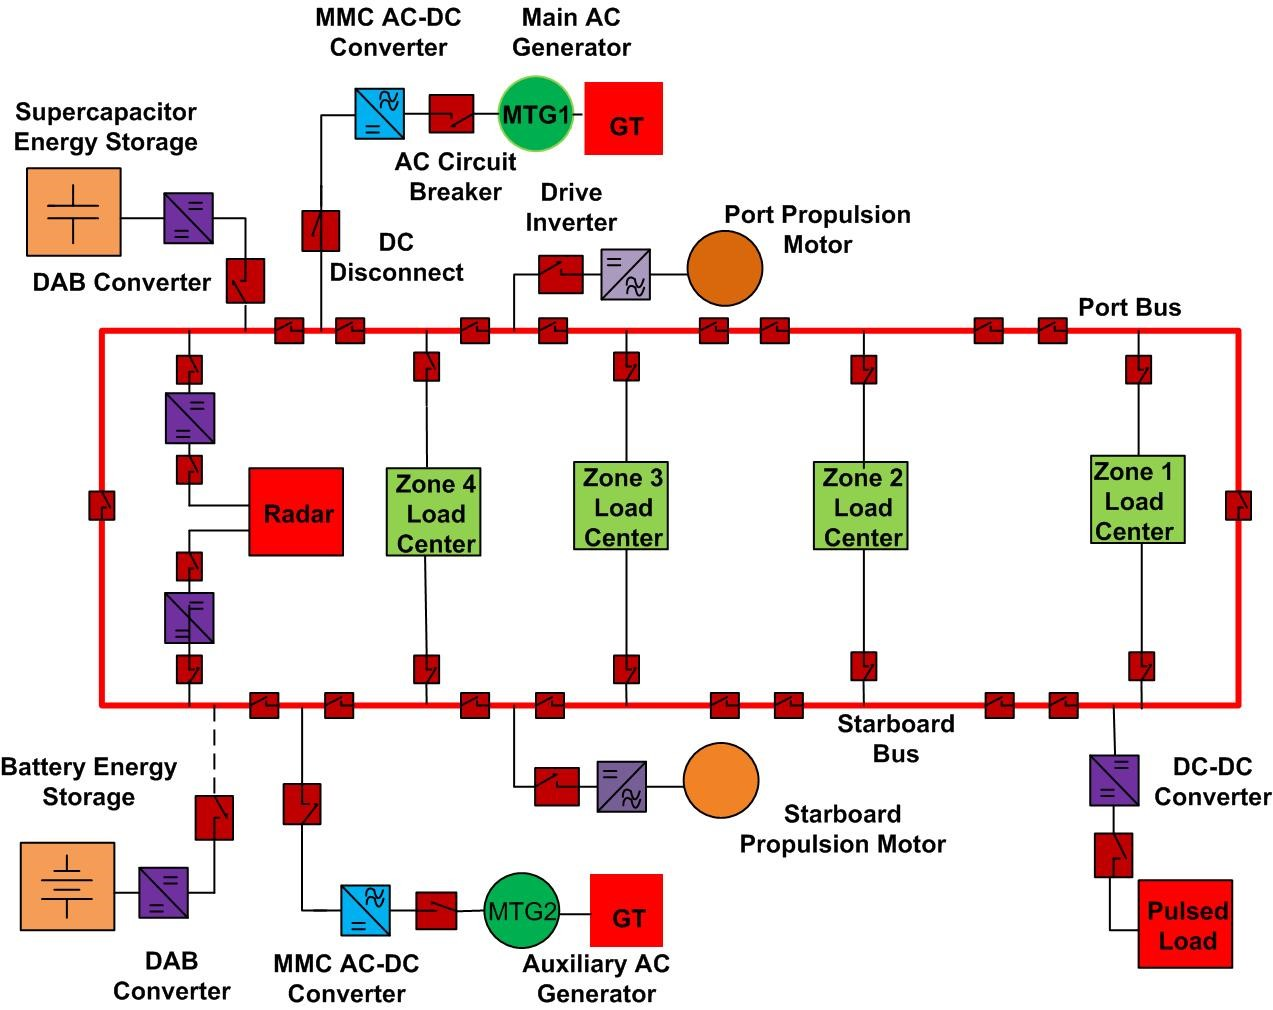
\includegraphics[width=\columnwidth]{f1}

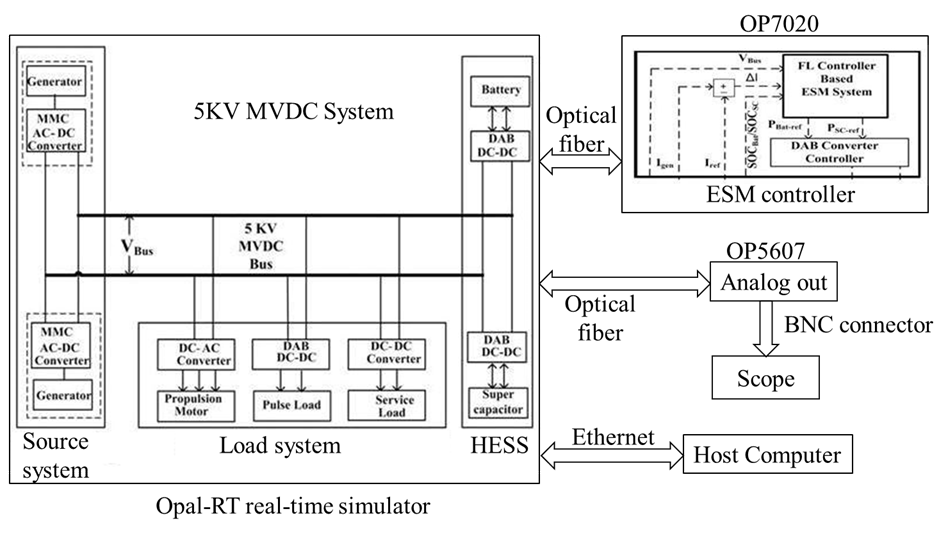
\includegraphics[width=3.5in]{f1111}
\caption{Block diagram of hardware setup for CHIL simulation of FL based ESM system.}
\label{ch5_f111}
\end{figure}

\begin{figure}[ht!]
\begin{subfigure}{1\columnwidth}
\begin{center}
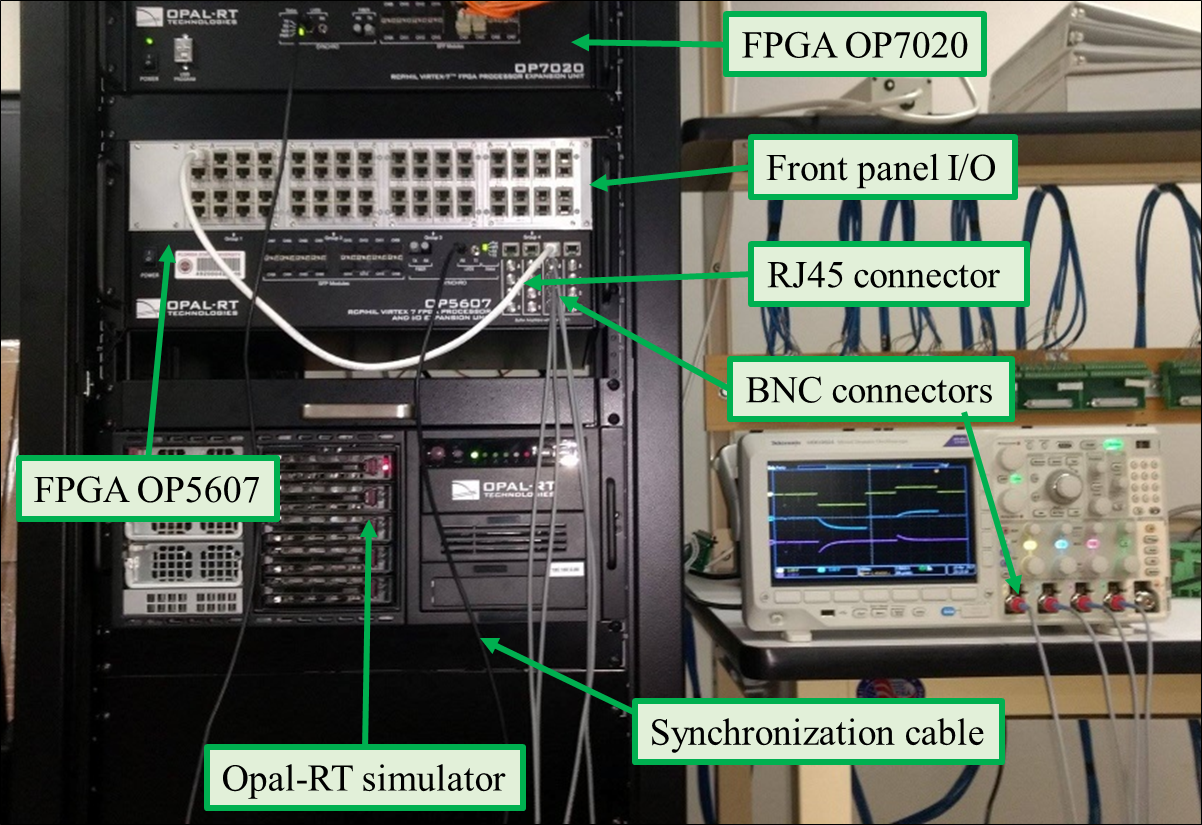
\includegraphics[height=1.9in, width=3.46in]{f112a}
\end{center}
\caption{Front panel.}
\label{ch5_f112a}
\end{subfigure}
\begin{subfigure}{1\columnwidth}
\begin{center}
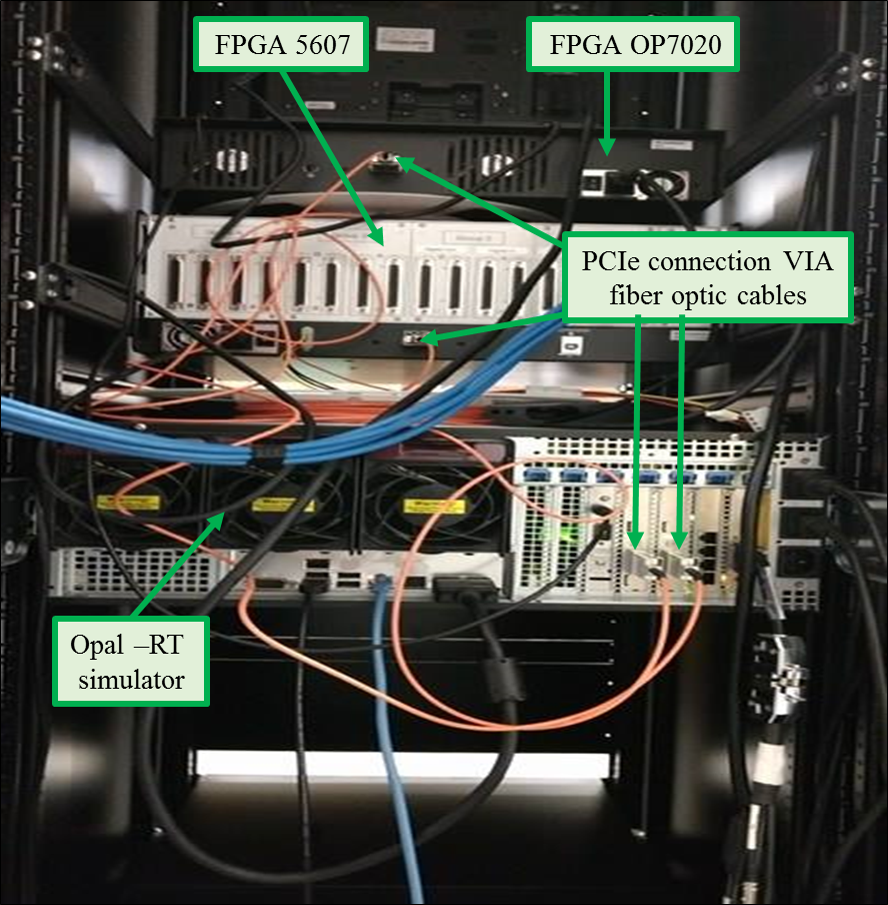
\includegraphics[height=2.05in, width=3.46in]{f112b}
\end{center}
\caption{Back panel.}
\label{ch5_f112b}
\end{subfigure}
\caption{Experimental setup for CHIL operation of FL based ESM system.}
\label{ch5_f112}
\end{figure}

\section{Results And Analysis}
An offline simulation of the FL control was carried out in \cite{khan2017fuzzy}.
In this section, the off-line and CHIL results are compared to validate the the performances of the FL controller based ESM system. 
\subsection{System Parameters}
Major parameters \cite{mystandard, andrus2015notional} used for the testing are listed in Table \ref{simulation-setup-table1} and Table \ref{simulation-setup-table10}. 
\begin{table}[ht!]
\centering
\processtable{The Simple Notional MVDC System Parameters \label{simulation-setup-table1}}
{\begin{tabu}{p{0.6cm}|p{2.9cm}|p{0.8cm}|p{0.6cm}|p{0.6cm}}
\hline
Type&Name&Quantity& P (MW) &$ P_{tot}$ (MW)\\
\hline
\multirow{2}{*}{Source} & MTG & 1& 36 & \multirow{2}{*}{40} \\  \cmidrule{2-4}
{}& ATG & 1& 4&\\
\hline
 \multirow{2}{*}{Load} & Normal Loads (Propulsion load, service loads and radar load) && 40  & \multirow{2}{*}{44} \\ 
\cmidrule{2-4}
 {}& Pulsed Load  & 1 & 4&\\ 
\hline
\end{tabu}}{}
\end{table}



%simulation parameters
\begin{table}[ht!]
\centering
\caption{Battery and Supercapacitor Parameters}
\label{simulation-setup-table10}
\begin{tabular}{p{2.5cm}|p{0.9cm}|p{2cm}|p{0.9cm}}
\hline
\multicolumn{2}{c|}{Battery} & \multicolumn{2}{c}{Supercapacitor} \\
\cmidrule{1-4}
Parameters & Values & Parameters & Values \\
\cmidrule{1-4} 
Rated capacity & 800Ah & Rated capacitance & 500.25F \\
\cmidrule{1-4}
Nominal voltage & 800V & Rated voltage & 550V \\
\cmidrule{1-4}
\cmidrule{1-4}
Fully charged voltage & 931.18V & Initial voltage & 465V \\
\cmidrule{1-4}
Initial SOC & 75\% & Initial SOC & 82.65\% \\
\cmidrule{1-4}

\end{tabular}
\end{table}
%\input{4a_2}
\subsection{Case 1: When SOC is within the limit (30\% $\leq$ SOC $\leq$ 90\%)}
For this case, the SOC of the battery and supercapacitor are set at 75\% and 82.65\%. 


At $t$ = 0.3s, 34MW load is connected to the MVDC system. With the addition of the load, bus voltage decreases momentarily and  the total load current increases. Fig. \ref{ch5_f113} shows the MVDC bus voltage and the total load current (off-line and CHIL). For this transient operation, the FL controller based ESM system provides total storage reference power ($P_{stor-ref}$) , the battery referance power and the supercapacitor referance power. The battery and supercapacitor reference power ($P_{Bat-ref}$ and $P_{SC-ref}$) are sent to the controllers of the DAB converters. At $t$ = 0.6s, another 6MW load is connected to the MVDC system. The total load of the system is now 40MW. Fig. \ref{ch5_f114} shows that the FL controller generate negative $P_{stor-ref}$ for discharging and the LPF separates the $P_{stor-ref}$  into $P_{Bat-ref}$  and $P_{SC-ref}$. At $t$ = 1s, 4MW pulsed load is added to the MVDC system and it is continued for $t$ = 2s. With the addition of pulsed load, total power demand (44MW) exceeds the total generation capacity (40MW) and the FL controller based ESM system provides nearly 4.5MW as $P_{stor-ref}$ for discharging (Figure \ref{ch5_f114}). Figure \ref{ch5_f115} shows the actual power response of the battery and supercapacitor. At $t$ = 2.5s, 4MW load is rejected and the FL controller based ESM system provides  positive $P_{stor-ref}$ for charging (Figure \ref{ch5_f114}).  Figure \ref{ch5_f115} shows the actual power consumed by the HESS. From the figures (Figure \ref{ch5_f113}, Figure \ref{ch5_f114}, and Figure \ref{ch5_f115}) it is clear that the Off-line and CHIL results are same. 


\begin{figure}[ht!]
\begin{subfigure}{1\columnwidth}
\begin{center}
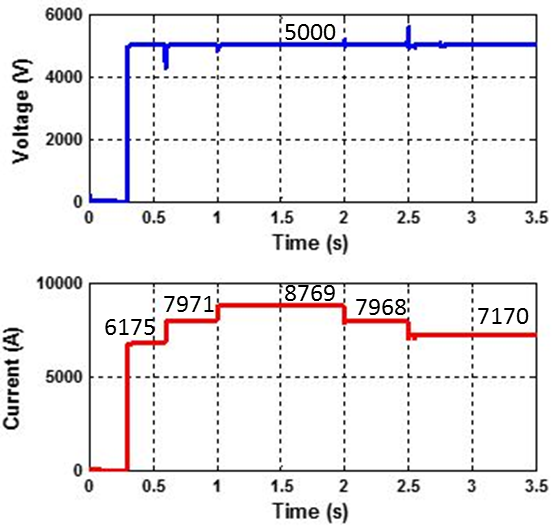
\includegraphics[height=3in, width=3.5in]{f113b}
\end{center}
\caption{Off-line simulation results.}
\label{ch5_f113b}
\end{subfigure}
\begin{subfigure}{1\columnwidth}
\begin{center}
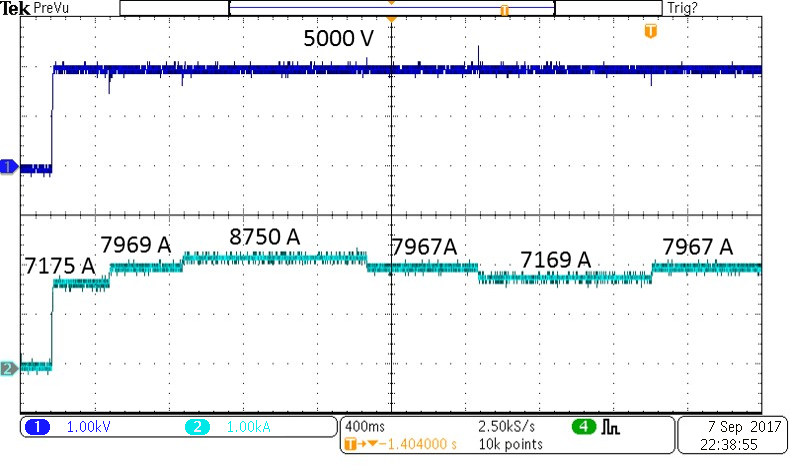
\includegraphics[height=2in, width=3.5in]{f113}
\end{center}
\caption{CHIL results-oscilloscope plots: Ch1: MVDC bus voltage and Ch2: total load current (Ch1: 2.5kV/div, Ch2: 4000A/div).}
\label{ch5_f113a}
\end{subfigure}
\caption{MVDC bus voltage and total load current (case 1).}
\label{ch5_f113}
\end{figure}
%gfhgfhfgjhg
%fghgfhg
\begin{figure}[ht!]
\begin{subfigure}{1\columnwidth}
\begin{center}
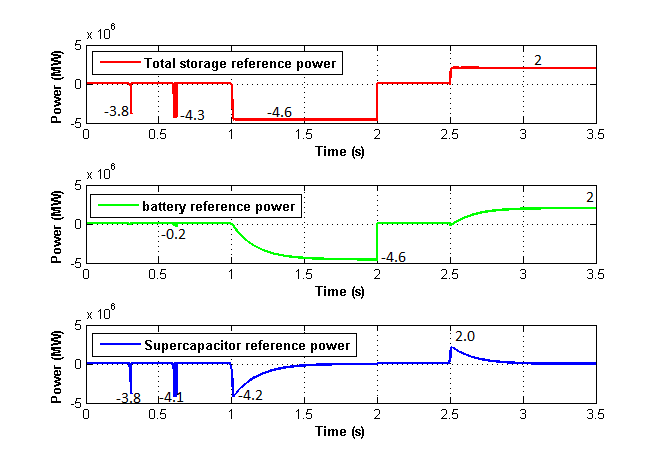
\includegraphics[height=3in, width=3.5in]{f114b}
\end{center}
\caption{Off-line simulation results.}
\label{ch5_f114b}
\end{subfigure}
\begin{subfigure}{1\columnwidth}
\begin{center}
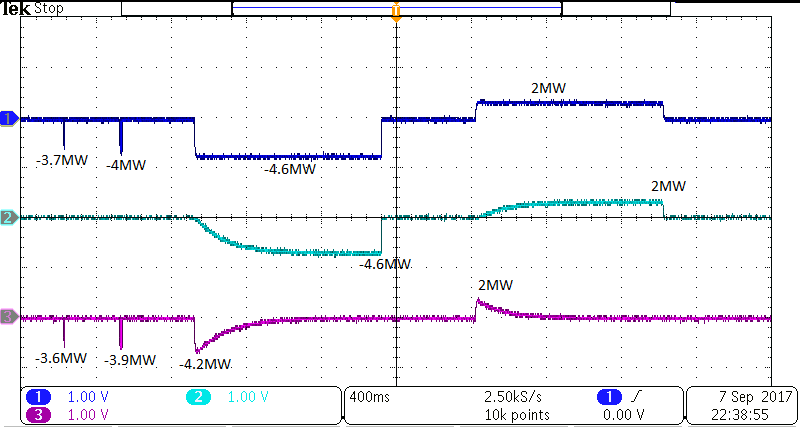
\includegraphics[height=2in, width=3.5in]{f114}
\end{center}
\caption{CHIL results-oscilloscope plots: Ch1: total storage reference power, Ch2: battery reference power, Ch3: supercapacitor reference  power (Ch1, Ch2, Ch3 = 5MW/div).}
\label{ch5_f114a}
\end{subfigure}
\caption{Reference power produced by FL controller and LPF based ESM system (case 1).}
\label{ch5_f114}
\end{figure}
%fdhgfhfgjh
%rfhgfhgfjhgjgh
%gfhgfhfgjhg
%fghgfhg
\begin{figure}[ht!]
\begin{subfigure}{1\columnwidth}
\begin{center}
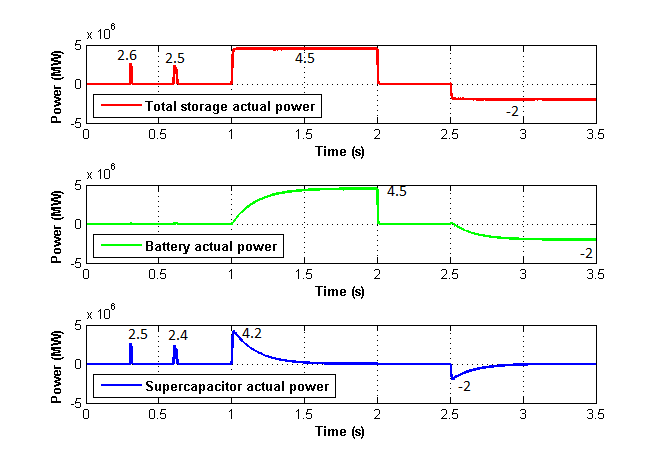
\includegraphics[height=3in, width=3.5in]{f115b}
\end{center}
\caption{Off-line simulation results.}
\label{ch5_f115b}
\end{subfigure}
\begin{subfigure}{1\columnwidth}
\begin{center}
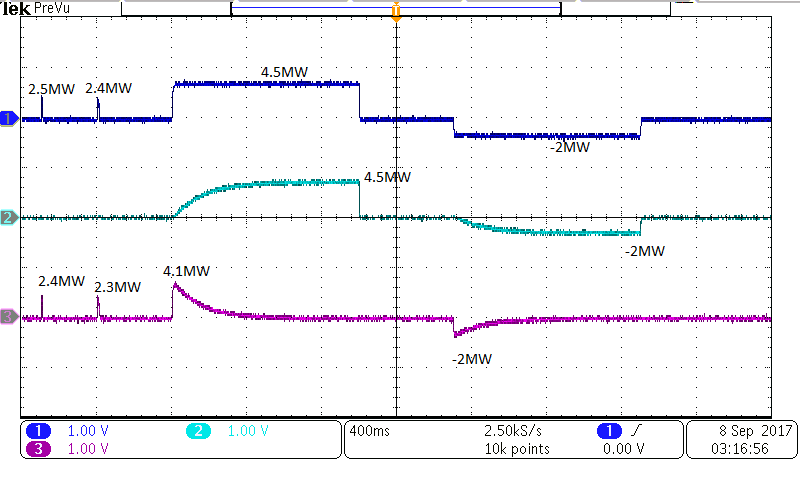
\includegraphics[height=2in, width=3.5in]{f115}
\end{center}
\caption{CHIL results-oscilloscope plots: Ch1: total storage actual power, Ch2: battery actual power, Ch3: supercapacitor actual power (Ch1, Ch2, Ch3 = 5MW/div).}
\label{ch5_f115a}
\end{subfigure}
\caption{Actual power response of the HESS (case 1).}
\label{ch5_f115}
\end{figure}
\subsection{Case 2: When SOC is below the limit}
In this case, the SOC of the battery is set at 20\% as the initial SOC and the supercapacitor’s initial voltage is kept 170V with SOC of 25.2\%. These voltages are below acceptable limit. Steps similar to case 1 are also performed here.  At $t$ = 0.3s and $t$ = 0.6s, 34MW and 6MW load are connected to the MVDC system, respectively. At $t$ = 1s, 4MW pulsed load is added to the MVDC system and it is continued until $t$ = 2s. With the addition of pulsed load, the total load (44MW) of the system exceeds the total generation capacity (40MW). Considering those operations, it is expected that the FL controller based ESM system will provide the negative $P_{stor-ref}$ for discharging. But from Fig. \ref{ch5_f116}, the FL controller based ESM system provides zero $P_{stor-ref}$. This is because, the reference power generation by the FL controller based ESM system also depends on the SOC of the battery and supercapacitor ($SOC_{Bat}$, $SOC_{SC}$) with the other two input variables, $\Delta I$ and $V_{Bus}$. Due to low SOC (20\% and 25.2\%),  the FL controller based ESM system provides zero reference power. Simulation results after $t$ = 2s are the same as shown in case 1, where at $t$ = 2.5s, 4MW load is the battery and supercapacitor start charging and continue until $t$ = 3.5s.
\begin{figure}[ht!]
\begin{subfigure}{1\columnwidth}
\begin{center}
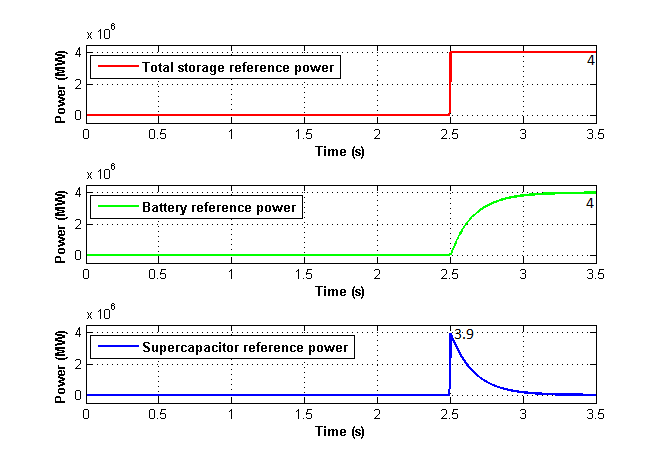
\includegraphics[height=3in, width=3.5in]{f116b}
\end{center}
\caption{Off-line simulation results.}
\label{ch5_f116b}
\end{subfigure}
\begin{subfigure}{1\columnwidth}
\begin{center}
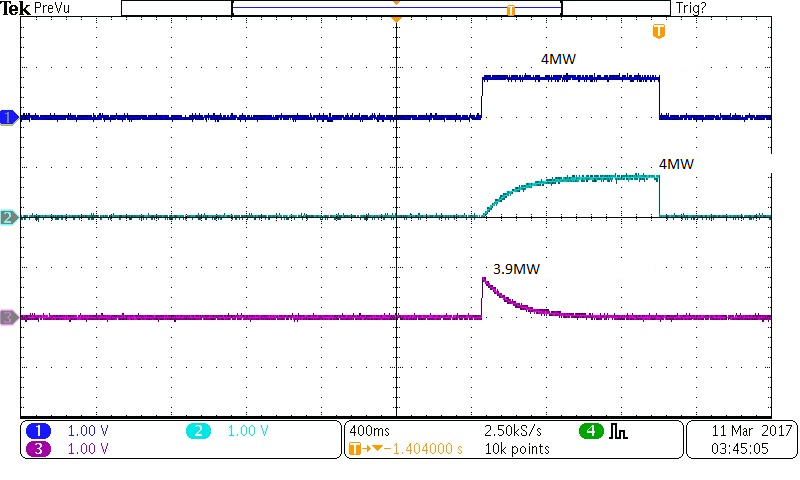
\includegraphics[height=2in, width=3.5in]{f116}
\end{center}
\caption{CHIL results-oscilloscope plots: Ch1: total storage reference power, Ch2: battery reference power, Ch3: supercapacitor reference  power (Ch1, Ch2, Ch3 = 5MW/div).}
\label{ch5_f116a}
\end{subfigure}
\caption{Reference power produced by FL controller and LPF based ESM system (case 2).}
\label{ch5_f116}
\end{figure}

\subsection{Case 3: When SOC is above the limit}
In this case, the SOC of the battery is set at 94\% as the initial SOC and the supercapacitor’s initial voltage is kept 535V with SOC of 97.02\%.

In this case, the same steps of the case 1 and case 2 are performed. From Fig. \ref{ch5_f117}, the simulation results up to $t$ = 2s  are the same as shown earlier in case 1, whereas at $t$ = 0.3s, $t$ = 0.6s and $t$ = 1s to $t$ = 2s,  34MW, 6MW and 4MW pulsed load are connected to MVDC system, respectively. From Fig. \ref{ch5_f117}, the FL controller based ESM system provides negative $P_{stor-ref}$ for discharging of the battery and supercapacitor and to supply power to the MVDC system. At $t$ = 2.5s, 4MW load is rejected and the FL controller based ESM system is expected to provide the positive $P_{stor-ref}$ for charging. But from Fig. \ref{ch5_f117}, the charging reference power ($P_{stor-ref}$) generated by the FL controller based ESM system is zero. This is because the reference power generation by the FL controller based EMS system depends on the SOC of the battery and supercapacitor with other two input variables. Due to the high SOC (nearly 94\% and 97.02\%) of the battery and supercapacitor, Fig. \ref{ch5_f117} shows that the FL controller based ESM system provides zero reference power for charging to avoid overcharging. From the Figure \ref{ch5_f117}, it is clear that the Off-line and CHIL results are same. 
  
%gfhgfhfgjhg
%fghgfhg
\begin{figure}[ht!]
\begin{subfigure}{1\columnwidth}
\begin{center}
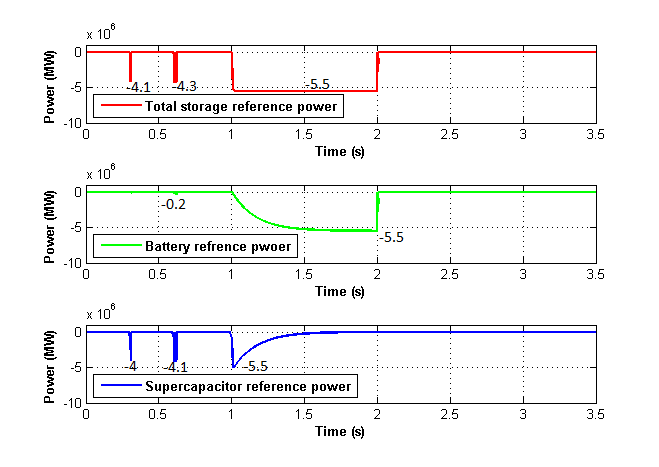
\includegraphics[height=3in, width=3.5in]{f117b}
\end{center}
\caption{Off-line simulation results.}
\label{ch5_f117b}
\end{subfigure}
\begin{subfigure}{1\columnwidth}
\begin{center}
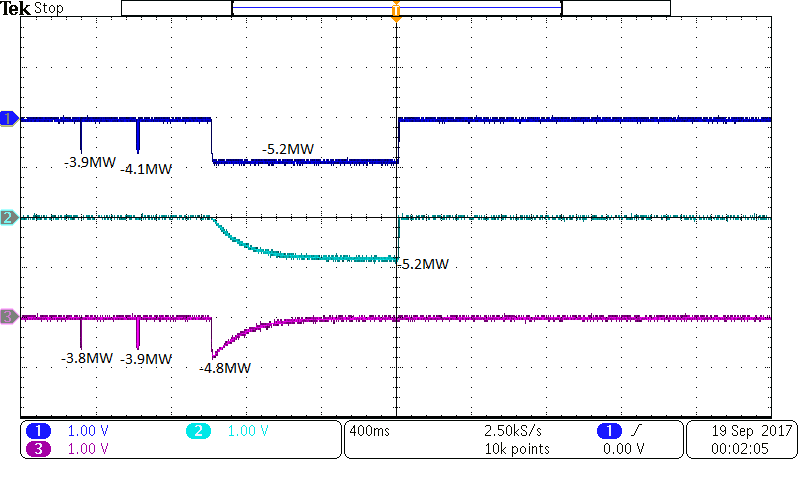
\includegraphics[height=2in, width=3.5in]{f117}
\end{center}
\caption{CHIL results-oscilloscope plots: Ch1: total storage reference power, Ch2: battery reference power, Ch3: supercapacitor reference  power (Ch1, Ch2, Ch3 = 5MW/div).}
\label{ch5_f117a}
\end{subfigure}
\caption{Reference power produced by FL controller and LPF based ESM system (case 3).}
\label{ch5_f117}
\end{figure}





%\input{7_comparison_of_fl_and_pi}
\section{Conclusion}
In this paper a FL based ESM is tested and validated using CHIL experiment. The MVDC system is modeled and simulated in a a DRTS whereas the control was implemented on FPGA. The HESS consisted of a battery and a supercapacitor is used to support the generators in meeting transient and steady power demand. A FL based intelligent ESM system is designed to control the power transfer among the energy storages and the MVDC system. The ESM system is implemented on Xilinx Virtex-7 FPGA (OP7020). Another FPGA board (OP5607) is used to show the analog output signals. CHIL based experiment is performed and the results are captured on the scope. Eventually, the CHIL based test results and off-line results from SimPowerSystems are compared. The results show that the FL based ESM is capable of maintaining the operations of the energy storages and assisting the generators in maintaining the power quality of the MVDC system.   




\section*{Acknowledgment}
This material is based upon research supported by or in part by, the US Office of Naval Research under award number N00014-16-1-2956.

\bibliographystyle{iet}
\bibliography{mybibi2}

\end{document}


